\documentclass[12pt]{article}
%% \usepackage{color} enabled in preamble
\usepackage[normalem]{ulem}  %% enable \st{} strikethrough

% This version hides the annotations so that the rendered PDF does not highlight the changes made in this revision
\usepackage[]{authblk}
\usepackage{graphicx}
\usepackage{tabularx}
\usepackage{color}
\usepackage{colortbl}
\usepackage[usenames,dvipsnames,table]{xcolor}
\usepackage{booktabs}
\usepackage{longtable}
\usepackage{hanging}
\usepackage{indentfirst}
\usepackage{setspace}
\usepackage{enumitem}
\usepackage{verbatim}
\usepackage{upgreek}
\usepackage{framed}
\usepackage{ textcomp }
\usepackage{url}
\usepackage{soul}
\usepackage{amsmath, amsfonts,amssymb,mathrsfs}
\usepackage{fancyhdr}
\usepackage[compact]{titlesec}
\usepackage[T1]{fontenc}
\usepackage{lmodern}
\usepackage{float}

%\usepackage[backend=bibtex,hyperref=true,citestyle=authoryear,bibstyle=authortitle,firstinits=true,terseinits=true,doi=false,url=false,maxbibnames=10,maxcitenames=2]{biblatex}
%\addbibresource{../bib_tex/master_refs.bib}


\usepackage[sectionbib]{chapterbib}
\usepackage[sectionbib]{natbib}

%\input{../bib_tex/biblatex_macros}


\setlength{\evensidemargin}{0in}
\setlength{\headheight}{0in}
\setlength{\headsep}{0in}
\setlength{\oddsidemargin}{-0.25in}
\setlength{\paperheight}{11in}
\setlength{\paperwidth}{8.5in}
\setlength{\tabcolsep}{0in}
\setlength{\textheight}{9in}
\setlength{\textwidth}{7in}
\setlength{\topmargin}{0in}
\setlength{\topskip}{0in}
\setlength{\voffset}{0in}
\parskip = 0.15in
\pagestyle{plain}
\setlength{\parindent}{0cm}

\definecolor{citescol}{RGB}{194,101,1}
\definecolor{urlscol}{RGB}{0,150,206}
\definecolor{linkscol}{RGB}{149,0,207}
\definecolor{mycol}{RGB}{25,23,191}
\definecolor{outputcol}{RGB}{34,139,34}
\definecolor{tcol}{RGB}{165,0,14}


\DeclareMathAlphabet{\msfsl}{T1}{cmr}{m}{it}
\DeclareMathAlphabet{\msyf}{OMX}{pcr}{m}{it}
\newcommand{\alf}{\upalpha}
\newcommand{\hilight}[1]{\colorbox{yellow}{#1}}

\newcommand{\levelone}[1]{
\bigskip
\noindent{\LARGE{\textsc{#1}}}
\vspace {0.05in}
}

\newcommand{\leveltwo}[1]{
\bigskip
\noindent{\Large{\textit{#1}}}
\vspace {-1mm}
}

\newcommand{\descriptionhead}[1]{
\noindent{\textbf{\textit{#1}}}\\ \vspace{-7mm}
}

\newcommand{\dhead}[1]{
\noindent{\textbf{\textit{#1 --}}}
}


\newcommand{\exs}[1]{
\vspace{-4mm}
\begin{itemize}
\item #1 \\ \vspace{-8mm}
\end{itemize}
}

\newcommand{\nbo}[1]{{\color{red}{#1}}}


\newcommand{\stepbullet}{\noindent \textbullet \ }
\newcommand{\mi}[1]{\textbf{\textit{#1}}}


\newcommand{\levelthree}[1]{\textit{#1 --}}


%\bibliographystyle{apalike}
%\bibpunct[; ]{(}{)}{;}{a}{,}{;}


\usepackage[breaklinks]{hyperref}
\usepackage[all]{hypcap}
\hypersetup{colorlinks=true,linkcolor=linkscol,citecolor=linkscol,urlcolor=urlscol}


% Abbreviations
\usepackage{xspace}
\newcommand{\IE}{{\it i.e.,}\xspace}
\newcommand{\EG}{{\it e.g.,}\xspace}
\newcommand{\CF}{{\it cf.}\xspace}
\newcommand{\IID}{i.i.d.\xspace}

\newcommand{\BAMM}{\texttt{BAMM}\xspace}
\newcommand{\BEAST}{\texttt{BEAST}\xspace}
\newcommand{\DDD}{\texttt{DDD}\xspace}
\newcommand{\diversitree}{\texttt{diversitree}\xspace}
\newcommand{\FigTree}{\texttt{FigTree}\xspace}
\newcommand{\Laser}{\texttt{laser}\xspace}
\newcommand{\MrBayes}{\texttt{MrBayes}\xspace}
\newcommand{\PAML}{\texttt{PAML}\xspace}
\newcommand{\PBD}{\texttt{PBD}\xspace}
\newcommand{\PhyloBayes}{\texttt{PhyloBayes}\xspace}
\newcommand{\Phylowood}{\texttt{Phylowood}\xspace}
\newcommand{\R}{\texttt{R}\xspace}
\newcommand{\Rev}{\texttt{Rev}\xspace}
\newcommand{\RevBayes}{\texttt{RevBayes}\xspace}
\newcommand{\TESS}{\texttt{TESS}\xspace}
\newcommand{\Tracer}{\texttt{Tracer}\xspace}
\newcommand{\TreePar}{\texttt{TreePar}\xspace}


\let\otheriint\iint
\let\iint\relax
\usepackage{ wasysym }

\usepackage{framed}
\usepackage[]{listings}
%\usepackage{fontspec}
\usepackage{placeins}
\usepackage{epstopdf}
\usepackage{scrextend}

\lstset{breaklines=true}

\lstdefinestyle{textboxSmall}{
  language=Matlab,
  stepnumber=1,
  numbersep=10pt,
  tabsize=4,
  showspaces=false,
  showstringspaces=false
}

%\definecolor{shadecolor}{RGB}{238,224,229}
%\definecolor{shadecolor}{RGB}{135,206,250}
\definecolor{shadecolor}{RGB}{183,207,237}

\setlength{\tabcolsep}{5pt}
\setlength{\topmargin}{-0.4in}
\setlength{\headheight}{14.5pt}
\pagestyle{plain}

\newcommand{\taha}[1]{{\textcolor{red}{[TAH comment: #1]}}} % TAH comment
\newcommand{\sdesc}[1]{
  \begin{addmargin}[1em]{0em}
    \textit{#1}
  \end{addmargin}
}



\definecolor{shcommentcol}{RGB}{0,0,255}
\definecolor{outlinecol}{RGB}{25,100,25}

\newcommand{\todo}[1]{\textcolor{red}{\textit{#1}}}
\newcommand{\blue}[1]{\textcolor{blue}{\textbf{#1}}}
\newcommand\marginal[1]{\marginpar{\raggedright\parindent=0pt\tiny #1}}

\newcommand{\outline}[1]{{\color{outlinecol}{\textbf{\textit{\large #1\\}}}}}

\newcommand{\shcomm}[1]{{\color{shcommentcol}{Sebastian: #1}}} % SH comments will be a soothing blue color

\newcommand\add[1]{{\color{black}{#1}}}
\newcommand\del[1]{}
%\newcommand\delm[1]{{\color{orange}{#1}}}
\newcommand\rep[2]{{\color{black}{#2}}}

\renewcommand\thesection{Protocol \arabic{section}}

\titlespacing{\section}{0pt}{*0}{*0}
\titlespacing{\subsection}{0pt}{*0}{*0}
\titlespacing{\subsubsection}{0pt}{*0}{*0}

\titleformat{\section}
  {\bigskip
  \normalfont\Large\bfseries\color{mycol}}
  {\thesection}{1em}{}

\titleformat{\subsection}
  {\medskip
  \normalfont\large\bfseries\color{black}}
  {\thesubsection}{1em}{}

\titleformat{\subsubsection}
  {\medskip
  \normalfont\bfseries\color{black}}
  {\thesubsubsection}{1em}{}

% command for MrBayes command-line step
\newcommand{\cl}[1]{{\texttt{\textbf{#1}}}}

\newcommand{\colx}[1]{{\textcolor{tcol}{#1}}}

\newcommand{\rbprmt}{ > }
\newcommand{\rbcl}[1]{\exs{\cl{\rbprmt{#1}}}}
\newcommand{\rbout}[1]{\cl{\textcolor{outputcol}{#1}}}
\newcommand{\rbdn}{{\Large \symbol{126}}} % This makes a copy/pasteable tilde
\newcommand{\rbclml}[1]{\exs{\cl{\ \ \ \ \ \ \ \ \ \ \ {#1}}}}



% text box settings
% requires compiling w/ XeLaTeX
%\newfontfamily\listingsfont[Scale=1.0]{Courier New}
%\lstset{basicstyle=\listingsfont, columns=texcl}
%\defaultfontfeatures{Mapping=tex-text}

%\lstset{columns=fullflexible}
%\lstset{basicstyle=\ttfamily,columns=flexible}
\lstdefinelanguage{Rev}
{morekeywords={RevBayes},
sensitive=false,
morecomment=[l]{\#},
moredelim=[il][\color{gray}\ttfamily]{|*},
}
%\lstdefinelanguage{Rev}
%{morecomment=[l]{#},
%moredelim=[il][\color{gray}\ttfamily]{|*},
%}
\lstset{
    language=Rev,
    basicstyle=\ttfamily,
    columns=flexible
}
%\lstset{morecomment=[l]{\#}}


% Some commands to keep the sysbio.bst from generating weird errors
\newcommand{\bibAnnoteFile}[1]{%
\IfFileExists{#1}{\begin{quotation}\noindent\textsc{Key:} #1\\
\textsc{Annotation:}\ \input{#1}\end{quotation}}{}}

\newcommand{\bibAnnote}[2]{%
\begin{quotation}\noindent\textsc{Key:} #1\\
\textsc{Annotation:}\ #2\end{quotation}}

\bibliographystyle{sysbio}
\bibpunct[; ]{(}{)}{;}{a}{}{;}



\makeatletter
\lst@CCPutMacro\lst@ProcessOther {"2D}{\lst@ttfamily{-{}}{-{}}}
\@empty\z@\@empty
\makeatother

% commands
\newcommand{\impmark}{\strut\vadjust{\domark}}
\newcommand{\domark}{%
  \vbox to 0pt{
    \kern-\dp\strutbox
    \smash{\llap{$\rightarrow$\kern1em}}
    \vss
  }%
}


%%\usepackage{fontspec}
%%\setmainfont{Times New Roman}
\usepackage{mathptmx}
\newcounter{proto}

% use 'rurl' to hide the 'http://' in text, but include it in the link
\newcommand\rurl[1]{%
	\href{http://#1}{\nolinkurl{#1}}%
}

% use 'button' to define a standard way to display clickable buttons
\newcommand\button[1]{%
	\textbf{#1}%
}

% use 'motif' to define a standard way to display motifs
\newcommand\motif[1]{%
    \textsc{\lowercase{#1}}%
}

% use 'uniprot' to define a standard way to display uniprot names
% TODO: HD/MG check if textsc/lowercase is the best way to represent this
\newcommand\uniprot[1]{%
	\textsc{\lowercase{#1}}%
}

% use 'fileformat' to define a standard way to display file formats
\newcommand\fileformat[1]{%
    \textit{#1}{}%
}%

\begin{document}


% Frontmatter

\thispagestyle{plain}
\begin{center}

\textbf{\LARGE \textit{Current Protocols in Bioinformatics}}\\\vspace{2mm}
\end{center}

\section*{Exploring Short Linear Motifs using the ELM Database and Tools}

{\small \it
Marc Gouw$^{1}$,
Hugo Samano$^{1}$,
Kim Van Roey$^{1}$,
Francesca Diella$^{1}$,
Toby J. Gibson$^{1}$,
Holger Dinkel$^{1,2}$

$^{1}$ Structural and Computational Biology Unit, European Molecular Biology
Laboratory, Meyerhofstrasse 1, 69117 Heidelberg, Germany\\
$^{2}$ Leibniz-Institute on Aging -- Fritz Lipmann Institute (FLI),
Beutenbergstrasse 11, 07745 Jena, Germany
}

\section*{Keywords}

Linear motifs, Bioinformatics, Protein-Protein Interaction, Molecular
switches, Cell regulation

\section*{Significance Statement}

Marc: TODO: still 23 words too long :(

Short Linear motifs (SLiMs) are small protein-interaction modules that play
essential roles in signalling, cell cycle progression, trafficking and disease.
SLiMs are short, often highly degenerate sequences with no stable
secondary structure, and have proven difficult to study both experimentally
and computationally.
It has been suggested that the number of different motifs in the
order of millions.
Yet, despite their abundance and importance, we have a very limited
understanding of which motifs exist and what they do.
The Eukaryotic Linear Motif (ELM) database is an online resource containing
over 3000 manually curated SLiMs from experimental
literature grouped into 262 motif classes.
This database can in turn be used to detect SLiMs in novel protein sequences.
ELM is a valuable resource to the scientific community studying protein
function, and will also play an important role in unravelling 
the complex nature of the biology.

% \emph{instructions: Provide a 120-word-maximum statement about the
% significance of the protocols/topic described in your manuscript. This
% should be understandable to undergraduate- educated scientists outside
% their field of specialty. The goal is to explain the relevance of the
% work in broad context to a broad readership. It will be used in
% promotion of the article following publication.}

\begin{abstract}%
%
% \emph{instructions: brief overview, no references, max 150 words}
%

Marc: TODO: this abstract is still pretty rough :(

The Eukaryotic Linear Motif (ELM) resource (\rurl{elm.eu.org}) is a
manually curated database of short linear motifs (SLiMs) as well as a tool to
detect and visualize motifs in protein sequences.

In this unit we will explore how to browse and search through the collection of
manually annotated data, and explain all of the different types of
knowledge and data integrated into the database.

We also cover how this resource can be used to search for SLiM's in novel
sequences, as well as giving examples of how to use the output of the ELM
prediction pipeline to evaluate which detections may be biologically relevant.

Lastly we also give examples of how the ELM database can be
searched as well queried programatically.

By the end of this unit the reader should have a much better understanding of
how to navigate the different content types contained in the database, as well
as how to use the ELM prediction pipeline for their own research.

\end{abstract}



% Introduction
\section*{Introduction}%
\label{sec:introduction}

The activity and function of a protein is tightly regulated by its
cellular environment. To interact with their surroundings, proteins use
various types of binding modules that each display distinct binding
properties \citep{10550212}. One prominent type of binding module
consists of short linear motifs (SLiMs) \citep{18508681}. These compact
binding sites are generally located in intrinsically disordered regions
(IDR) of the proteome and commonly bind to
surfaces of a globular domain of a protein \citep{21909575}. SLiMs mediate
different types of interactions that regulate protein functionality, and hence
are important regulators of the dynamic processes involved in cell
signalling \citep{22480932} \citep{24926813}. The number of
SLiM instances in the human proteome is currently suggested to be over
one million \citep{25038412}. Identifying SLiMs and elucidating their
functionality is an essential step in understanding cell regulation. The
Eukaryotic Linear Motif (ELM) resource contributes to this process by
providing the necessary tools to researchers working on motifs. It
consists of a database and a prediction tool. The database provides a
categorised repository of experimentally validated linear motif classes
and instances that were manually annotated from the literature. The ELM
prediction tool in turn relies on annotated data, both from the ELM
database and other resources, to accurately analyse unknown sequences
for candidate motifs and assist researchers in selecting the most
plausible ones for experimental validation and discard likely false
positive hits, saving them valuable time and resources \citep{22110040}.
The following protocols will guide users through the different ELM
applications, explaining how to browse the curated data available in
ELM, how to analyse a protein sequence for putative motifs, and how to
interpret these data and avoid common pitfalls in SLiM discovery.


% Browsing and exploring content
\section{Exploring the Content of the ELM Database}%
\label{sec:explore_content}%

% TODO: this paragraph is technically not part of the protocol but rather introduction
% I think this part is OK here: It introduces the annotated part of the database.
% Also, I think we can 'assume' that most Papers will be read from top to bottom?
The core of the ELM database is a repository of manually annotated motifs and
instances. As of January 2017, ELM contains over 260 motif classes and over
3000 experimentally validated and manually curated instances.
The motif classes and motif instances have been uploaded by a large group of
annotators from around the globe. The complete catalogue of manually curated
data can be searched, browsed and explored on the ELM website.

% TODO: this paragraph is technically not part of the protocol but rather introduction
% This part: agreed, if we can find a way to put it in the introduction.
% Although I don't think its too bad here :)
Each motif class describes a short linear motif, a short sequence of amino acids
with a dedicated function. Since the motifs are often degenerate, each motif
class is represented using ``regular expressions'': a symbolic representation
expressing a complex pattern of letters (or amino acids). For example, the
regular expression ``\motif{[FY].L.P}'' is to be read as: The first amino acid
is a Phenylalaline '\motif{F}' or a Tyrosine '\motif{Y}' followed by any one
amino acid '\motif{.}', a Leucine '\motif{L}', one more arbitrary amino acid
'\motif{.}' and finally a Proline '\motif{P}'.

% TODO: this paragraph is technically not part of the protocol but rather introduction
% I also think this part is a nice part for the introduction to this section
% (annotated data)
In all cases the annotator condenses information from the primary and secondary
literature into manageable abstracts, accompanies the motif definition with
a list of experimental instances, as well as links to external resources including
biological pathways, diseases, Gene Ontology and other protein resources. In
this protocol we explore the several data-types stored in the database, as well
as links to external resources.

%
% Subsection: Necessary Resources
%
\subsection*{Necessary Resources}
\subsubsection*{Software \& Hardware}
A modern browser such as Firefox, Chrome, or Safari. ELM is best viewed
on a laptop or desktop computer, although tablets and smartphones will
also work.



%
% Subsection: Database content overview
%
\subsection*{Database content overview}%
\label{subsec:explore_content_database}%


% Counter for steps
\begin{enumerate}%

%TODO: Improve/expand all captions

\begin{figure}[h!]%
	\centering%
	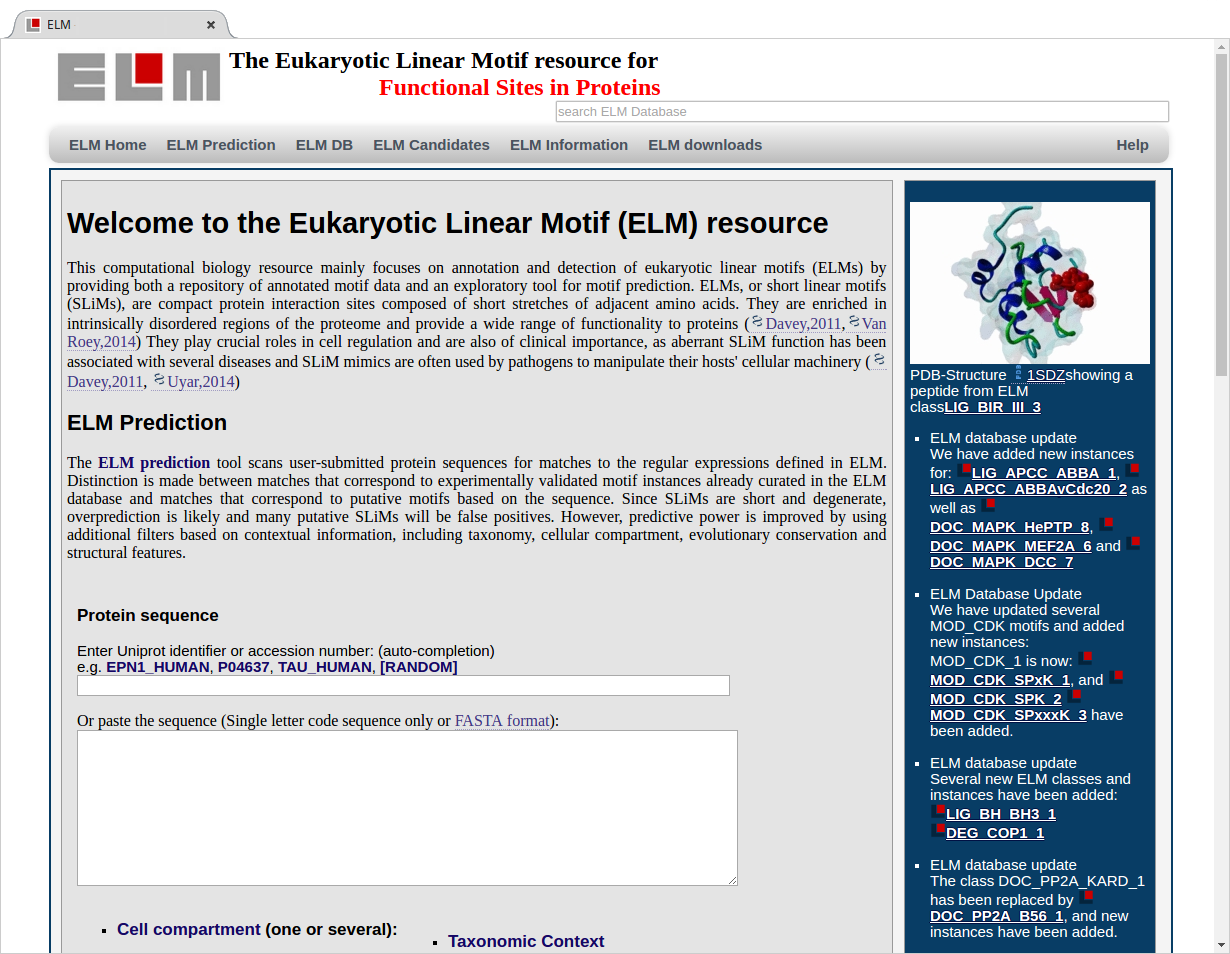
\includegraphics[width=\textwidth]{Figures/explore_content/home.png} %
	\caption{%
		The homepage of the ELM database (\rurl{elm.eu.org}).%
	}%
	\label{fig:explore_content_home}
\end{figure}

\item The ELM database is an online web resource. Open a browser and navigate
	to \rurl{elm.eu.org} to visit the homepage
	(Figure~\ref{fig:explore_content_home}).
	This page shows a brief explanation of the ELM resource, and a form to
	search for SLiMs (which we cover in further detail in
	\ref{sec:predicting_p53} and \ref{sec:predicting_cv_0974}).
	The column to the right is continually
	updated with the latest news about changes and additions to the database.

\begin{figure}[h!]
	\centering
	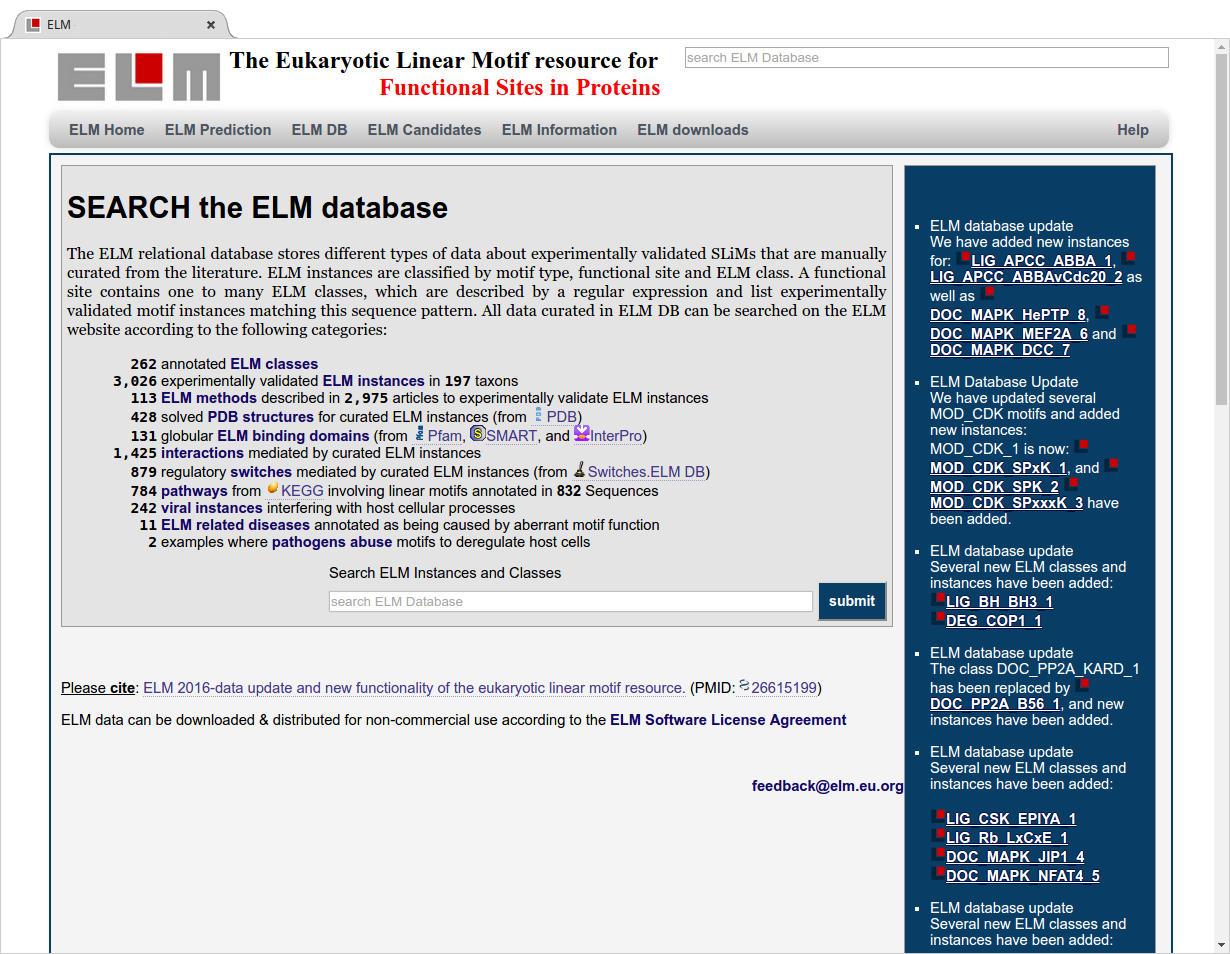
\includegraphics[width=\textwidth]{Figures/explore_content/stats.png}
	\caption{
		The ELM database statistics overview page shows the most up-to-date
		database statistics. As of January 2017, ELM has just over
		3000 annotated instances in 262 different motif classes.
	}
	\label{fig:explore_content_stats}
\end{figure}

\item On the ELM homepage click on the menu link \button{ELM DB} for an overview of
	the database statistics (Figure~\ref{fig:explore_content_stats}).
	This page displays the types and amounts of annotations contained in
	the database and a few links to third-part databases.
	Each line contains at least one link that will take you
	to the corresponding contents page.
	For example: Clicking on \button{ELM classes} will take you to the
	page showing all classes annotated in ELM.
	We will be exploring these content overview pages in this protocol.
% HD:I find the following sentence confusing, as the user doesn't know whether he should click on that 'instances' button or not... will be explained later anyways
%	(for example, clicking on
%	\button{ELM instances} will take you to the page displaying all of the
%	annotated instances in the database).
%
% Marc: I completley agree. I added some things which I hope makes it clearer.

%
% Subsection: Browsing motif classes and instances
%
\subsection*{Browsing motif classes and annotated instances}
\label{subsec:explore_content_classes_and_instances}

\begin{figure}[h!]
	\centering
	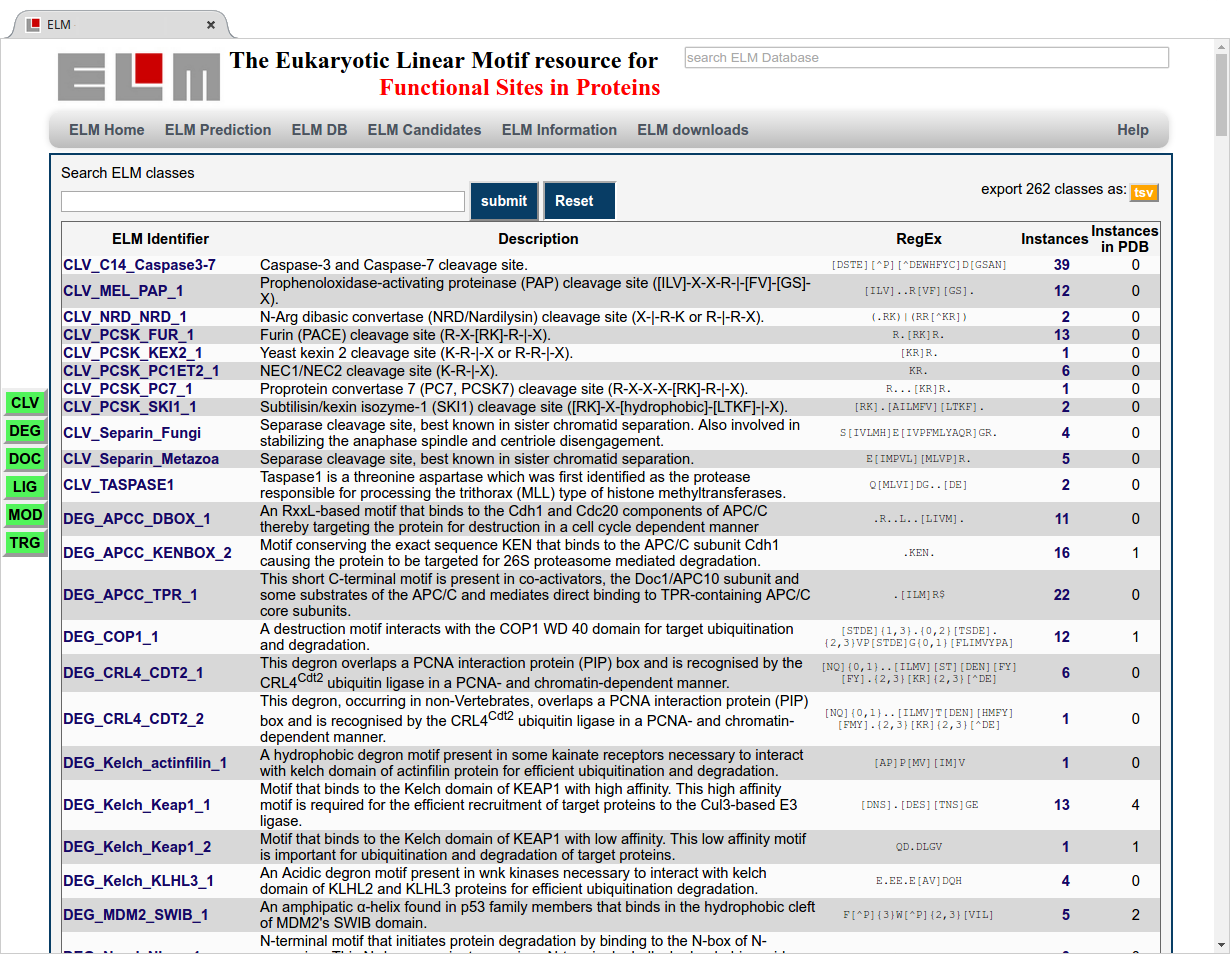
\includegraphics[width=\textwidth]{Figures/explore_content/elms.png}
	\caption{
		The list of all motif classes annotated in the ELM database.
	}
	\label{fig:explore_content_elms}
\end{figure}

\item Click on the sub-menu \button{ELM classes} under \button{ELM DB} to visit
	the page listing all of the ELM classes
	(Figure~\ref{fig:explore_content_elms}).
	For each class, the following information is provided: ELM identifier,
	short description, regular expression, number of instances annotated
	for each class, and number of structures available. For details on each
	class, click on the ELM identifier; to get a list of annotated
	instances for an individual class, click on the number of instances.

	\sdesc{Use the search bar at the top of the page to filter for certain
		motif classes. For example, typing ``MAPK'' and hitting \button{submit}
		will perform a full-text search on all motif classes in the ELM
		database containing the term ``MAPK''. The green buttons on the
		left can also be used to filter this table. For example,
		toggling the ``DOC'' button will remove all DOC classes
		from the table (and clicking it again will bring them back).
		Lastly, the yellow \button{tsv} link can be used to export all
		motif classes as a ``tab separated values'' file.}

\begin{figure}[h!]
	\centering
	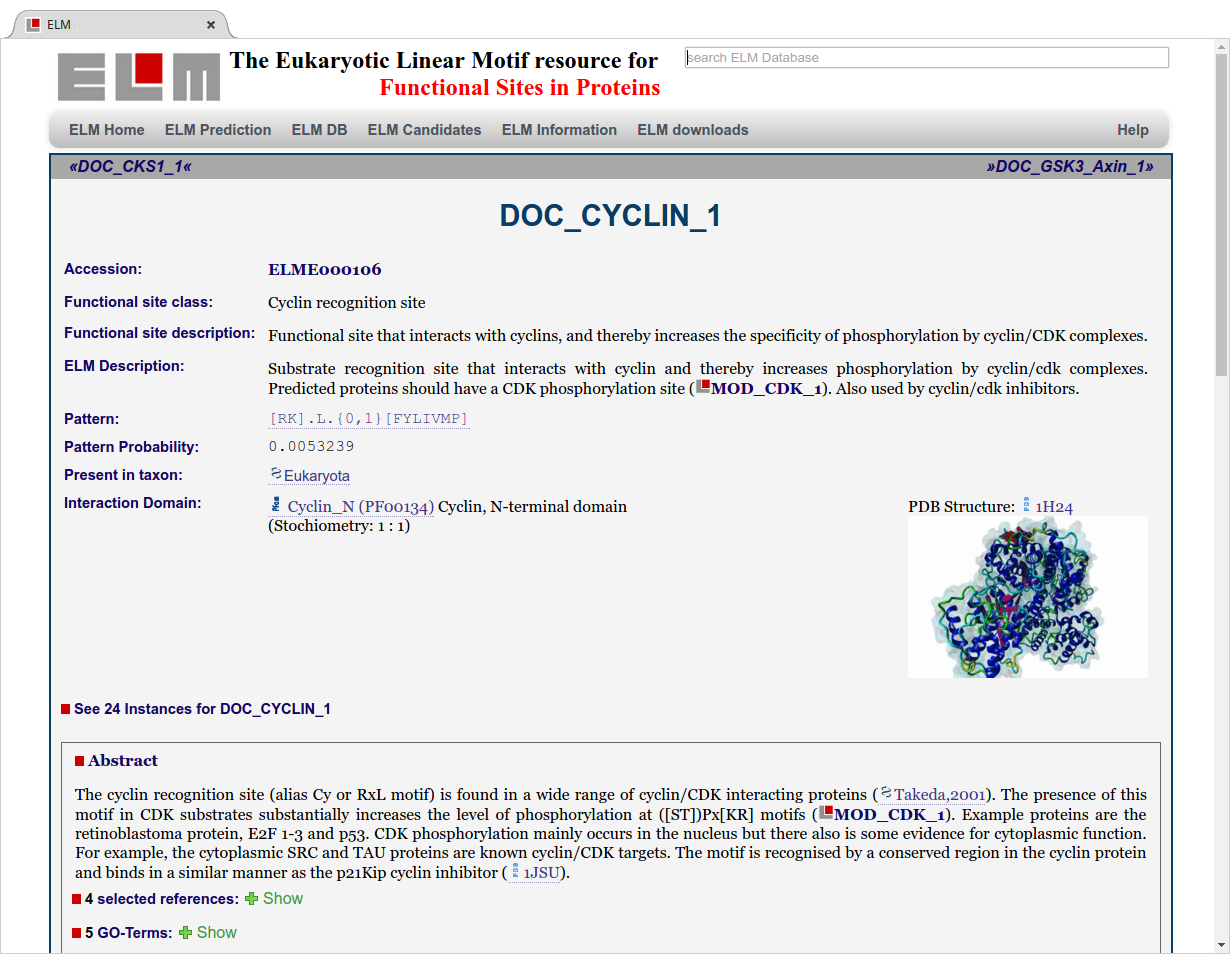
\includegraphics[width=\textwidth]{Figures/explore_content/doc_cyclin_1_class.png}
	\caption{
        The motif details page for \motif{DOC\_CYCLIN\_1}. This page
	contains all of the manual annotation details for the
    \motif{DOC\_CYCLIN\_1} motif, the biological background summarized from
	the scientific literature including links to the primary
	literature and to external resources (Pubmed \citep{27899561},
	the Gene Ontology \citep{27899567}, PDB \citep{12037327} and
	more).
	}
	\label{fig:explore_content_doc_cyclin}
\end{figure}

\item Search the table for the term \motif{DOC\_CYCLIN\_1} and click on
	\button{DOC\_CYCLIN\_1} in the left column to
	navigate to the page with details about the
	\motif{DOC\_CYCLIN\_1} motif class
	(Figure~\ref{fig:explore_content_doc_cyclin}).
	This page contains a description of the
	functional site class (a Cyclin recognition site), and a short
	description of the ELM and its regular expression, as well as a
	probability score, the taxonomic distribution of the motif and which
	domain (if any) is responsible for the interaction.

	\sdesc{The probability score is the probability that the regular
		expression represents a random selection of amino acids
		(similar to an information content score). A lower score
		indicates that the motif pattern is more difficult to find by
		chance in a random sequence.}

% TODO: Could explain more of the content, eg. Probability, interaction domain etc.
% TODO: be more consistent in using bold, italics, inverted-commas - it should be clear what are clickable links
\item Scroll further down the \motif{DOC\_CYCLIN\_1} page
	(Figure~\ref{fig:explore_content_doc_cyclin}) to view
	more details about this motif
    (Figure~\ref{fig:explore_content_doc_cyclin_1_abstract_instances})
    The ``abstract'' contains a description of the biological relevance of the
    motif (for example its involvement in cellular processes and pathways).
	annotation. Click on the \button{show} button next to the ``selected
	references'' header for a list of publications relevant to this motif.
	Click on \button{show} next to ``GO terms'' for a complete list of all
	Gene Ontology (GO) terms annotated for this motif.

\begin{figure}[h!]
	\centering
	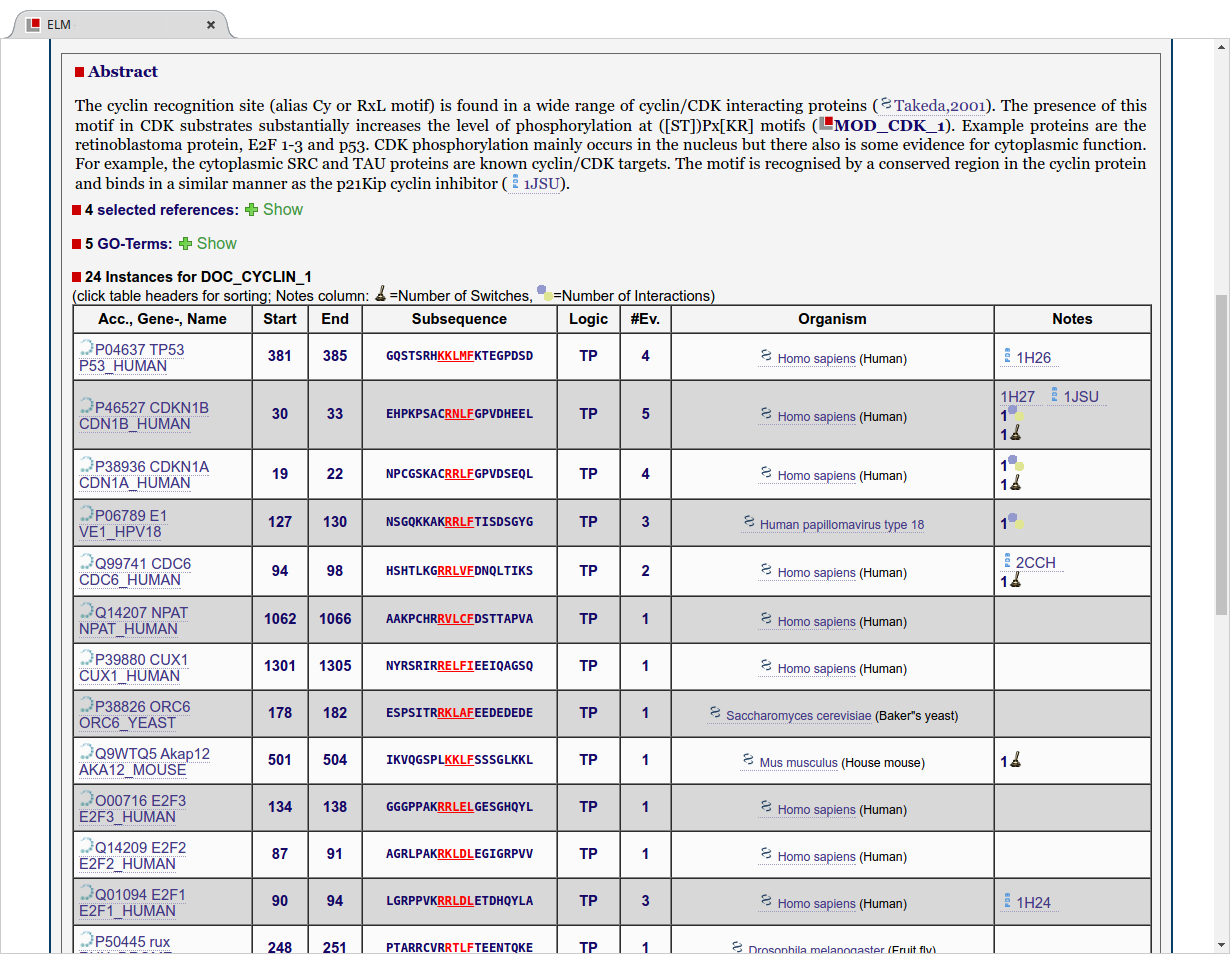
\includegraphics[width=\textwidth]{Figures/explore_content/doc_cyclin_1_abstract_instances.png}
	\caption{
		The second part of the \motif{DOC\_CYCLIN\_1} motif details page
		shows the motif abstract GO terms, and the list of annotated
		instances.
	}
	\label{fig:explore_content_doc_cyclin_1_abstract_instances}
\end{figure}

\item Scroll further down the \motif{DOC\_CYCLIN\_1} page to view
	the ``Instances'' header
	(Figure~\ref{fig:explore_content_doc_cyclin_1_abstract_instances})
	This table contains the list of all annotated \motif{DOC\_CYCLIN\_1}
	instances in the database of this motif. This includes the protein
	identifier, the start and end positions of the instance, the specific
	sequence matching the regular expression representing the motif and
	the ``logic'' of the instance.
	The ``\#~Ev.'' indicates the number of experimental evidences
	associated with the annotation. ``Organism'' indicates in which
	species in which the protein is found. Lastly the ``Notes'' column
	contains links to any ``interactions'' or ``switches'' present in the
	database, as well as links to PDB, if the structure exists in PDB.

	\sdesc{The instance ``logic'' is an annotation of whether this is a
		\textit{bona-fide} instance, or whether it is a non-functional
		instance. \textit{TP} (True positive) indicates the instance is
		annotated with experimental evidence showing, that it is functional.
		\textit{FP} (False Positive) instances have experimental
		evidence suggesting function, but are believed to be
		non-functional, after careful examination by our annotators.
		\textit{TN} (True Negative) instances have been experimentally
		determined to be non-functional, and \textit{U} (Unknown)
		instances do not have enough evidence to determine whether it
		is functional or not. The overwhelming majority of instances in
		ELM are \textit{TP}s.}


\begin{figure}[h!]
	\centering
	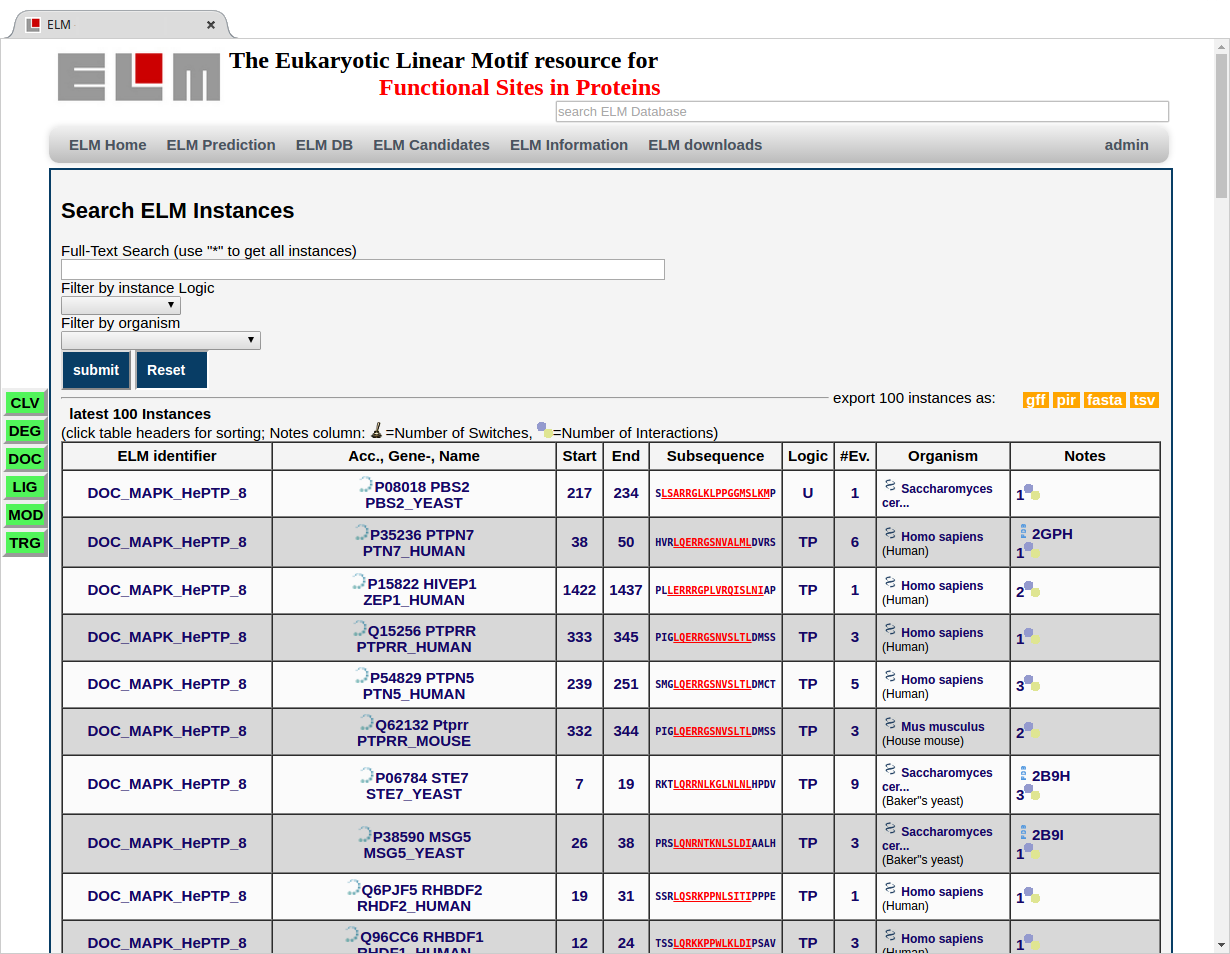
\includegraphics[width=\textwidth]{Figures/explore_content/instances.png}
	\caption{
		The ``instances'' page can be used to search for instances in
		the ELM database.
	}
	\label{fig:explore_content_instances}
\end{figure}

\item \label{sec:explore_content_instances} Click on the sub-menu \button{ELM instances} under \button{ELM DB} to visit
	the page where you can search and browse the instances annotated in ELM
	(Figure~\ref{fig:explore_content_instances}).
	Note that only the first hundred instances matching the search criteria are shown.
	The search form can be used to filter results by a full text search, by
	instance logic, or by organism.

% TODO: explain GFF, PIR, FASTA?
	\sdesc{This table can be filtered by motif class using the green toggle
		filters on the left hand side. Lastly, the yellow buttons at
		the top of the page can be used to download the instances in
		the following formats: \fileformat{GFF}, \fileformat{PIR},
		\fileformat{FASTA} or \fileformat{TSV}.}

\begin{figure}[h!]
	\centering
	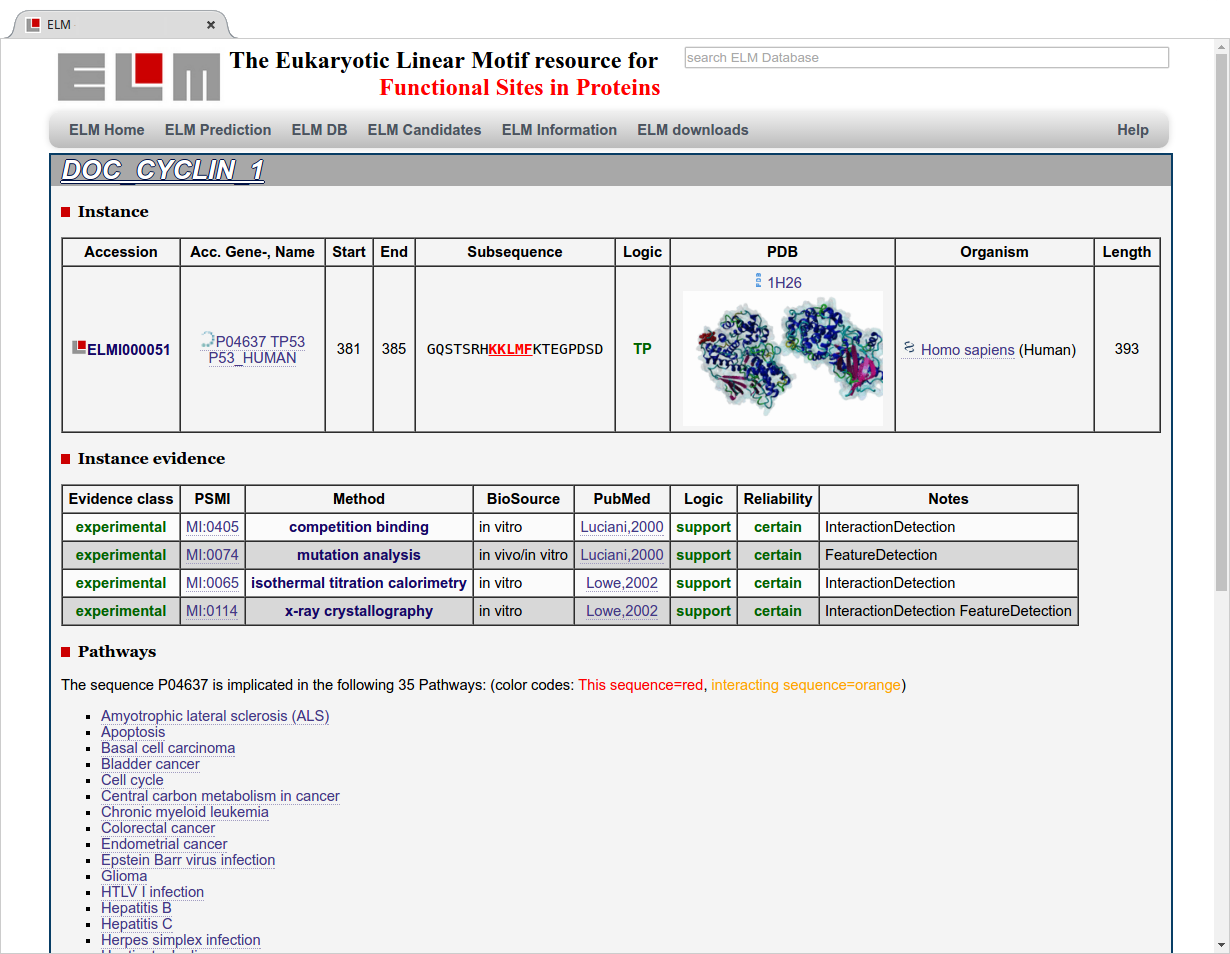
\includegraphics[width=\textwidth]{Figures/explore_content/doc_cyclin_1_instance.png}
	\caption{
	The instance details page for the \motif{DOC\_CYCLIN\_1} instance annotated
	for protein \uniprot{P53\_HUMAN} with start/end position ``381--385''. This page
	also contains links to many external databases including UniProt
	\citep{25348405}, PDB \citep{12037327}, NCBI taxonomy and Pubmed
	\citep{27899561}, and KEGG pathways \citep{26476454}, as well as the
	PSI-MI controlled vocabulary \citep{17925023}.
	}
	\label{fig:explore_content_doc_cyclin_instance}
\end{figure}

\item Type ``p53\_human'' in the search box to search for ELM Instances in this
	protein. Find the row for the ELM class \motif{DOC\_CYCLIN\_1} and click on
	the instance sub-sequence (highlighted in red) to go to the instance
	details page of this
	instance (Figure~\ref{fig:explore_content_doc_cyclin_instance}).
	The top part of the page contains details about the instance
	and the protein it was identified in, as well as a link to the UniProt entry for
	the protein \citep{25348405}.

\item Scroll down to the ``Instance Evidence'' header to view details on the
	experimental evidence used to annotate this instance. The each
	experimental method is annotated using the Proteomics Standards
	Initiative Method Identifier (PSI-MI) \citep{17925023}, as well as the
	references in which the experiments were published.

	\sdesc{
		The ``biosource'' indicates whether method is \emph{in vivo},
		\emph{in vitro}, \emph{in silico} or a combination of these.
		The ``logic'' column indicates whether this experiment
		supports or contradicts this instance being functional.
		Each method is also annotated with a reliability assessment, which can
		be any of certain, likely, unlikely or unspecified.}

%
% Subsection: Switches, pathways and other external resources.
%
\subsection*{Finding Switches and molecular interactions}
\label{subsec:explore_content_external_resoureces}

\begin{figure}[h!]
	\centering
	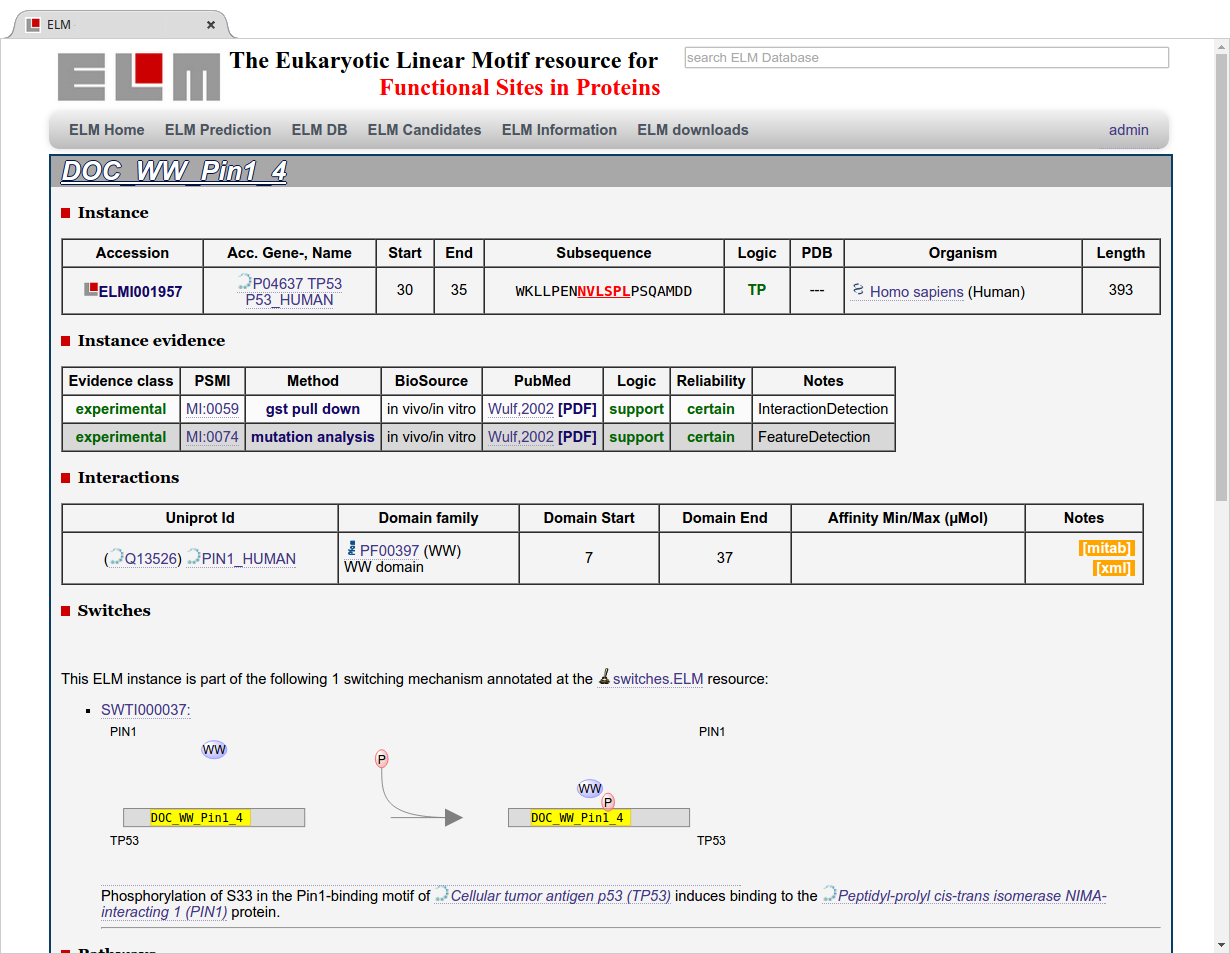
\includegraphics[width=\textwidth]{Figures/explore_content/doc_ww_pin_1_4_instance.png}
	\caption{
	The instance details page for the \motif{DOC\_WW\_Pin1\_4}
	instance found in human p53 (\uniprot{P53\_HUMAN}) with start/end position
	``30--35''.
	}
	\label{fig:explore_content_doc_ww_instance}
\end{figure}

\item Repeat the previous search by clicking on the sub-menu \button{ELM instances}
	under \button{ELM DB} and type ``p53\_human'' in the search box. This time,
	find the ELM instance of the motif \motif{DOC\_WW\_Pin1\_4} with the
	start/end position ``30--35''. (You can sort the table by clicking on the
	header lines: click on ``Start'' to sort by start position ). Click on the
	start/end position or the sub-sequence that will take you to the details
	page (Figure~\ref{fig:explore_content_doc_ww_instance}). This
	page is similar to that described for the p53 instance \motif{DOC\_CYCLIN\_1}
	(Figure~\ref{fig:explore_content_doc_cyclin_instance}).
	Additionally, for this instance, there is information available about
	its interaction partner and a molecular switch, which is mediated by
	this motif instance.

\item Scroll down to the ``Interactions'' header to view information about this
	instance's interactions
	(Fig.ure~\ref{fig:explore_content_doc_ww_instance}). This instance
	interacts with \uniprot{PIN1\_Human} via the ``WW'' domain (Pfam identifier
	PF00397; found on position 7--37 in \uniprot{PIN1\_Human}. If available,
	binding affinities are also shown here. Interaction data is made
	available in \fileformat{MiTab} and \fileformat{XML} format
	\citep{17925023}, and can be downloaded by clicking on the yellow
	buttons in the right column.

\item Scroll further down to the ``Switches'' section for a brief overview of
	the switches details of this instance obtained from "switches.ELM"
	\citep{23550212} (Figure~\ref{fig:explore_content_doc_ww_instance}). This
	particular instance is part of a phosphorylation-dependant molecular switch --
	only if p53 is phosphorylated on residue Serine-33 can it bind to the protein
	``Peptidyl-prolyl cis-trans isomerase NIMA-interacting 1 (PIN1)``.
	Clicking on the diagram will open an external link to the
	\rurl{switches.elm.eu.org} website where more detail can be found.

%
% Subsection: Links to external resources
%
\subsection*{Exploring Links to External Protein Resources}
\label{subsec:explore_content_links_to_external_resources}

\begin{figure}[h!]
	\centering
	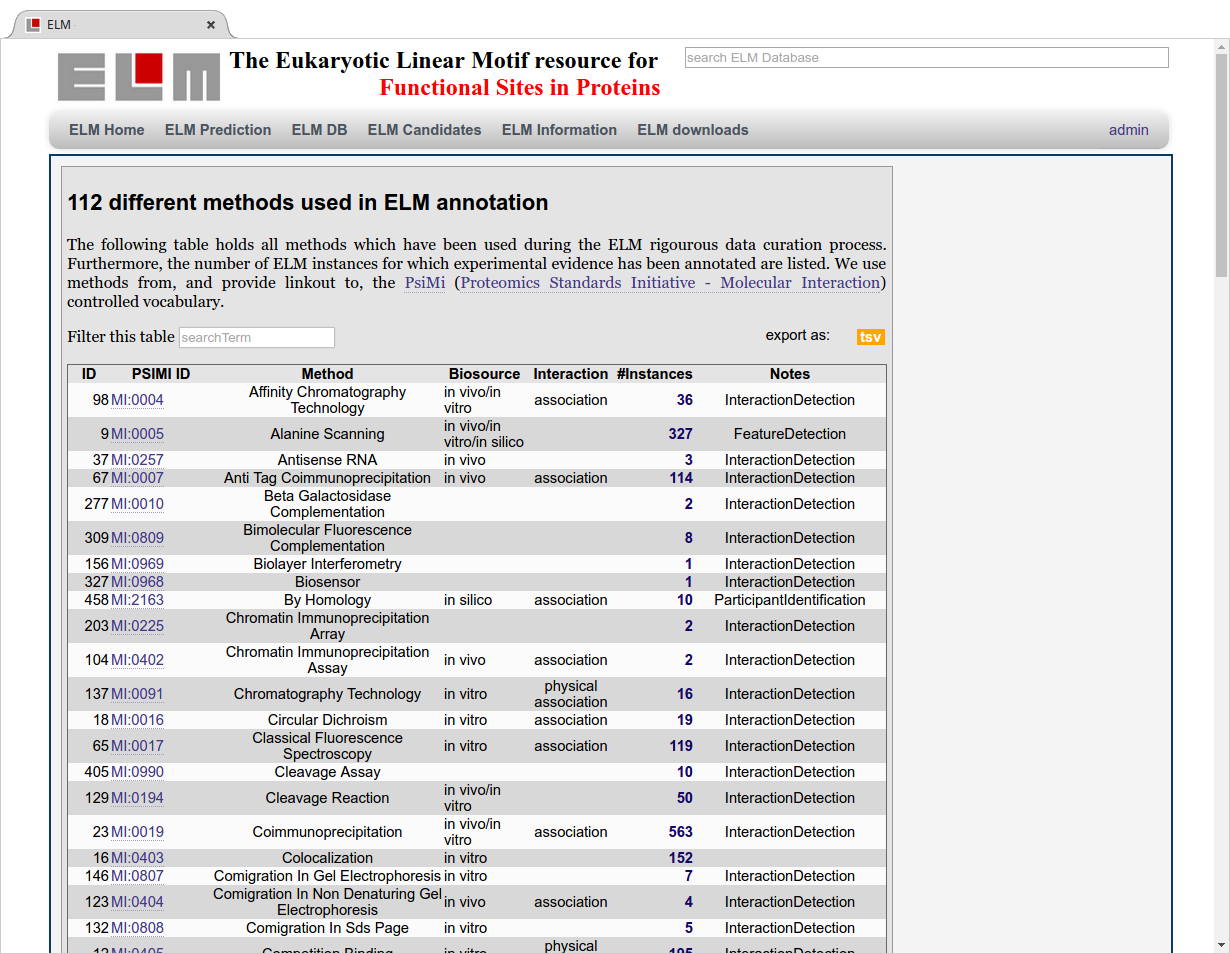
\includegraphics[width=\textwidth]{Figures/explore_content/methods.png}
	\caption{
		The list of all experimental methods used in the ELM database,
		along with their PSI-MI identifiers.
	}
	\label{fig:explore_content_methods}
\end{figure}

\item Click on the sub-menu \button{ELM methods} under \button{ELM DB} to see a
	list of all experimental methods, which have been used to identify
	motifs and instances (Figure~\ref{fig:explore_content_methods}).
	This table shows the internal method
	identifier in the first column, a link to the corresponding entry in
	the PSI-MI database \citep{17925023}, and the method name as annotated
	by the PSI-MI controlled vocabulary, as well as the type of experiment
	(\textit{in vitro}, \textit{in vivo}, \textit{in silico}, or a combination of these).
    Clicking on the link in the ``instances'' column
	will list all instances annotated using that method.

	\sdesc{The filter bar on the top page can be used to filter the list of
		methods. The \fileformat{TSV} link creates a downloadable file
		in ``tab separated values'' format.}

\begin{figure}[h!]
	\centering
	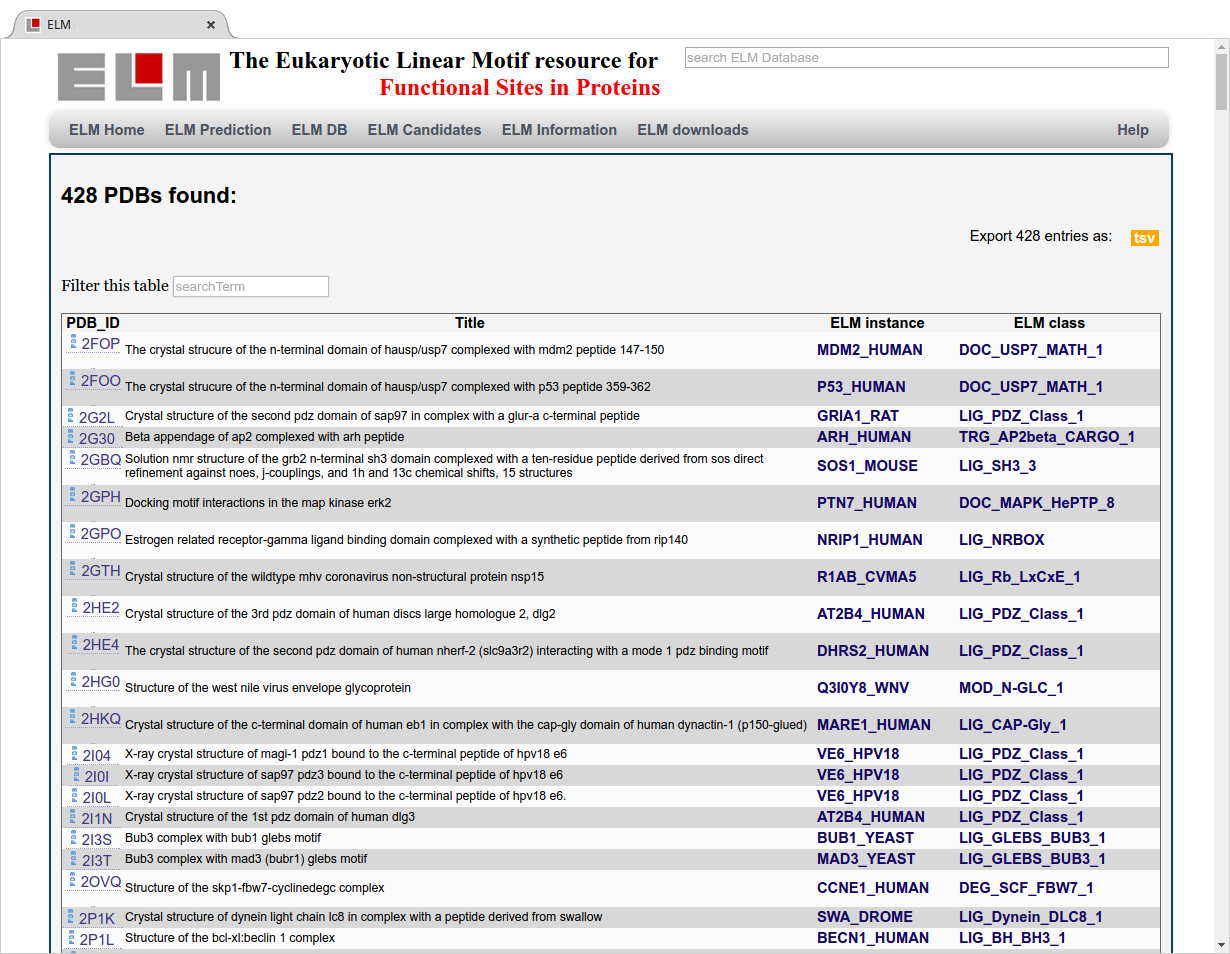
\includegraphics[width=\textwidth]{Figures/explore_content/pdbs.png}
	\caption{
	The list of all known PDB structures for which annotated motif instances exist in the ELM database.
	}
	\label{fig:explore_content_pdbs}
\end{figure}

\item Click on the sub-menu \button{ELM PDB structures} under \button{ELM DB} to
	see a list of all macromolecular structures in the ELM database
	(Figure~\ref{fig:explore_content_pdbs}).
	Structures annotated in ELM ideally (but not always) show
	both interaction partners (motif and domain). This page also contains
	links to RCSB/PDB \citep{12037327}, the individual instance and the motif
	class of that instance.

% duplicate information:
%	\sdesc{The filter bar on the top page can be used to filter the list of
%		structures shown. The yellow \fileformat{TSV} link creates a
%		downloadable file in ``tab separated values'' format.}

\begin{figure}[h!]
	\centering
	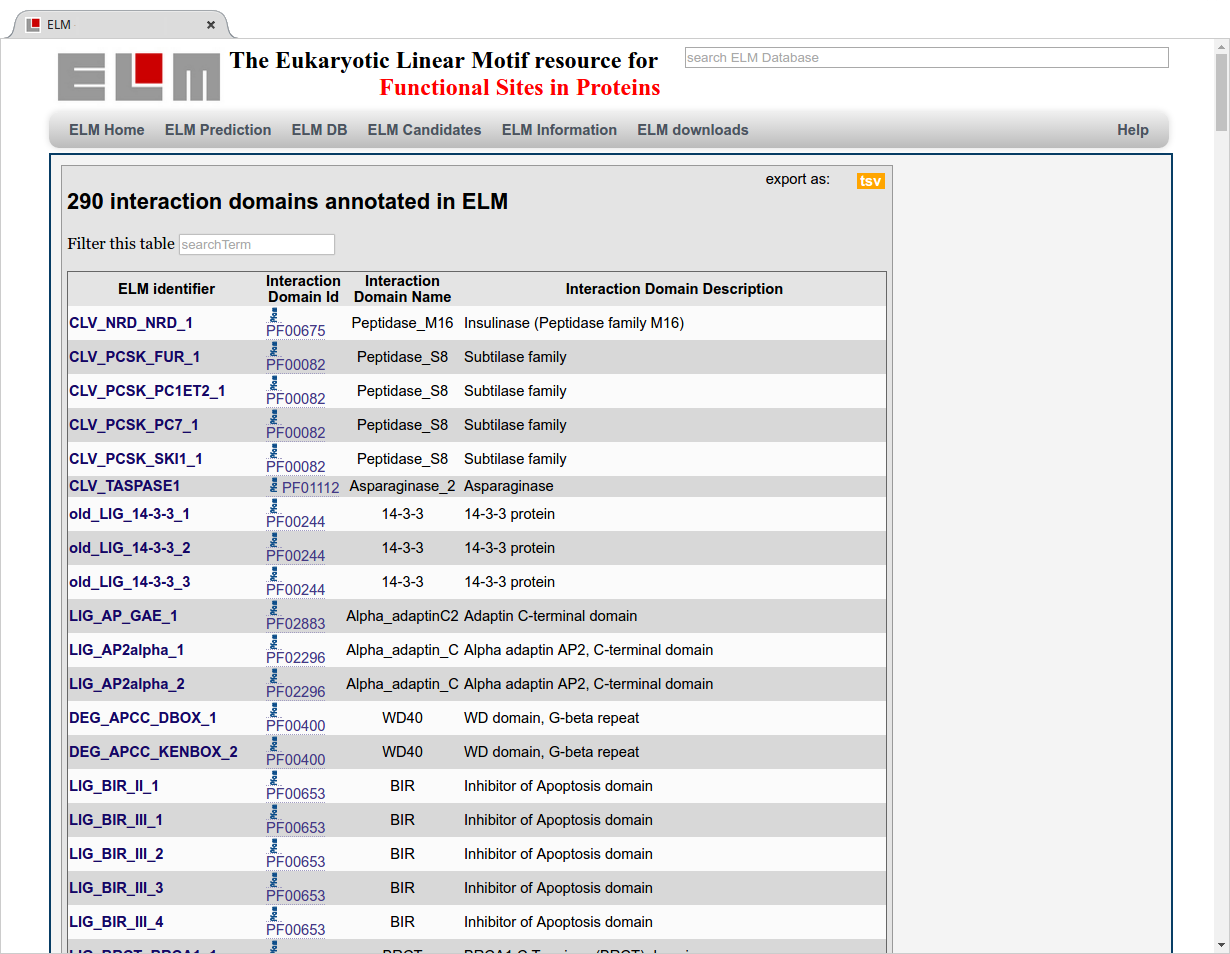
\includegraphics[width=\textwidth]{Figures/explore_content/interactiondomains.png}
	\caption{
	A list of all interactions annotated in the database.
	}
	\label{fig:explore_content_interaction_domains}
\end{figure}

\item Click on the sub-menu \button{ELM binding domains} under \button{ELM DB}
	to see a complete list of all the interaction domains in ELM
	(Figure~\ref{fig:explore_content_interaction_domains}).
	This table shows the ELM classes that have been annotated
	with a corresponding interaction domain divided by the ELM
	class, a link to the Pfam \citep{26673716}, SMART \citep{25300481} or
	InterPro \citep{27899635} domain, as well as the name of the
	interacting domain followed by a brief description.

% duplicate information:
%	\sdesc{The filter bar on the top page can be used to filter the list of
%		interactions shown. The \emph{tsv} link creates a downloadable
%		file in ``tab separated values'' format.}

%
\begin{figure}[h!]
	\centering
	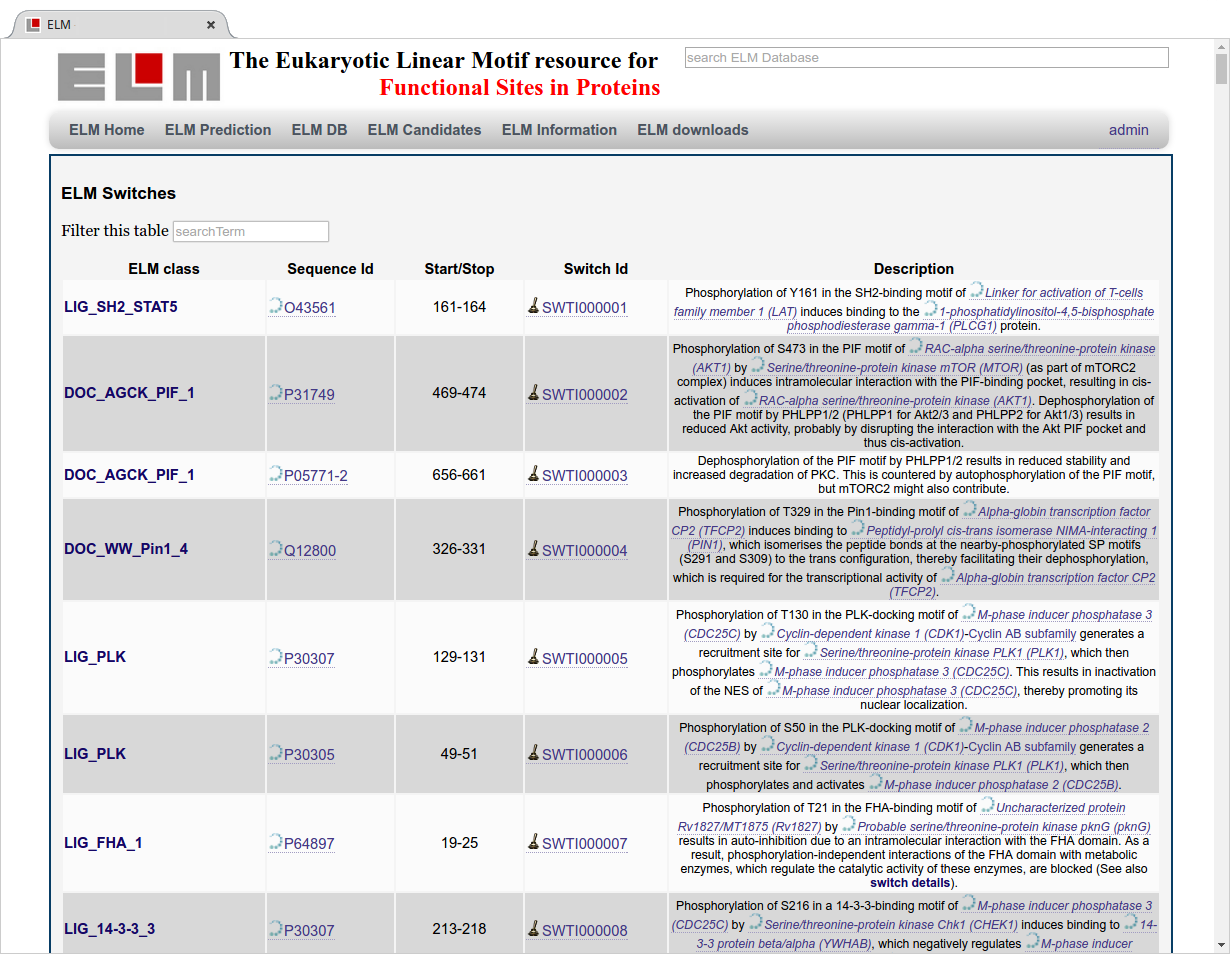
\includegraphics[width=\textwidth]{Figures/explore_content/switches.png}
	\caption{
	    A list of all molecular switches that are based on instances
	    from ELM and which are annotated at the \rurl{switches.elm.eu.org}
	    database.
	}
	\label{fig:explore_content_switches}
\end{figure}

\item Click on the sub-menu \button{ELM switches} under \button{ELM DB} to see a complete
	list of all the molecular switches annotated in ELM
	(Figure~\ref{fig:explore_content_switches}). This table shows
	the motif class, contains a link to UniProt, as well as the start and stop
	positions of the motif mediating the switch. The last two columns show
	links to the \rurl{switches.elm.eu.org} website, and a brief description
	of the switch (taken from the switches.ELM database, see \cite{23550212}).

% duplicate information:
%	\sdesc{The filter bar on the top page can be used to quickly filter
%		the list of interactions shown.}

%
% Subsection: Exploring KEGG pathways
%

\subsection*{Visualizing KEGG pathways from ELM}
\label{subsec:explore_content_kegg}

\begin{figure}[h!]
	\centering
	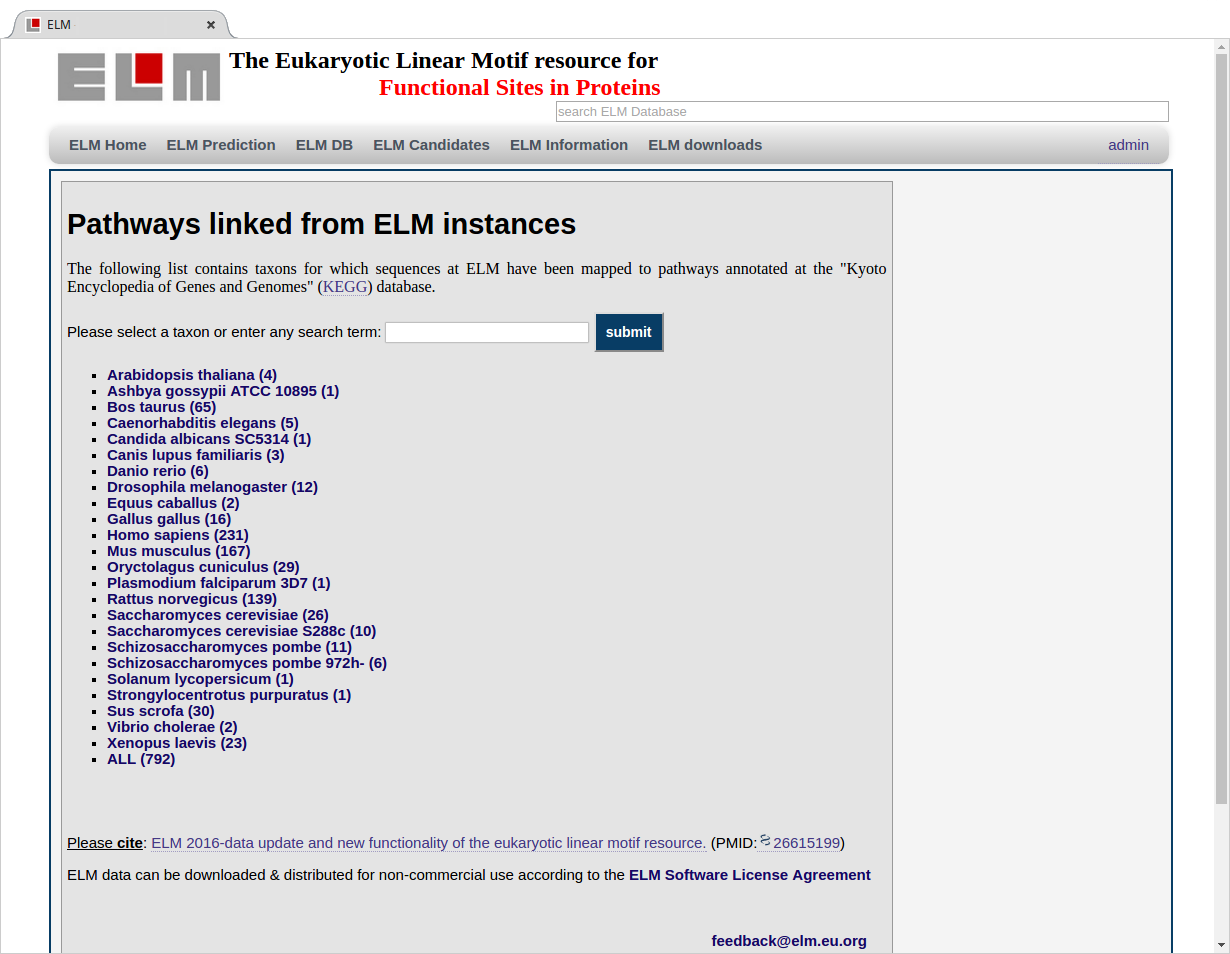
\includegraphics[width=\textwidth]{Figures/explore_content/pathways.png}
	\caption{
	    A list of organisms for which pathways from KEGG have been mapped to protein sequences of instances in ELM. The number in brackets
	    denotes the number of different pathways per organism.
	}
	\label{fig:explore_content_pathways}
\end{figure}

\item Click on the sub-menu \button{ELM pathways} under \button{ELM DB} to see a list of all
	KEGG pathways contained in ELM
	(Figure~\ref{fig:explore_content_pathways}).
	Pathways are taken from and mapped onto the ``Kyoto Encyclopedia of Genes and Genomes'' (KEGG
	\citep{26476454}).

\begin{figure}[h!]
	\centering
	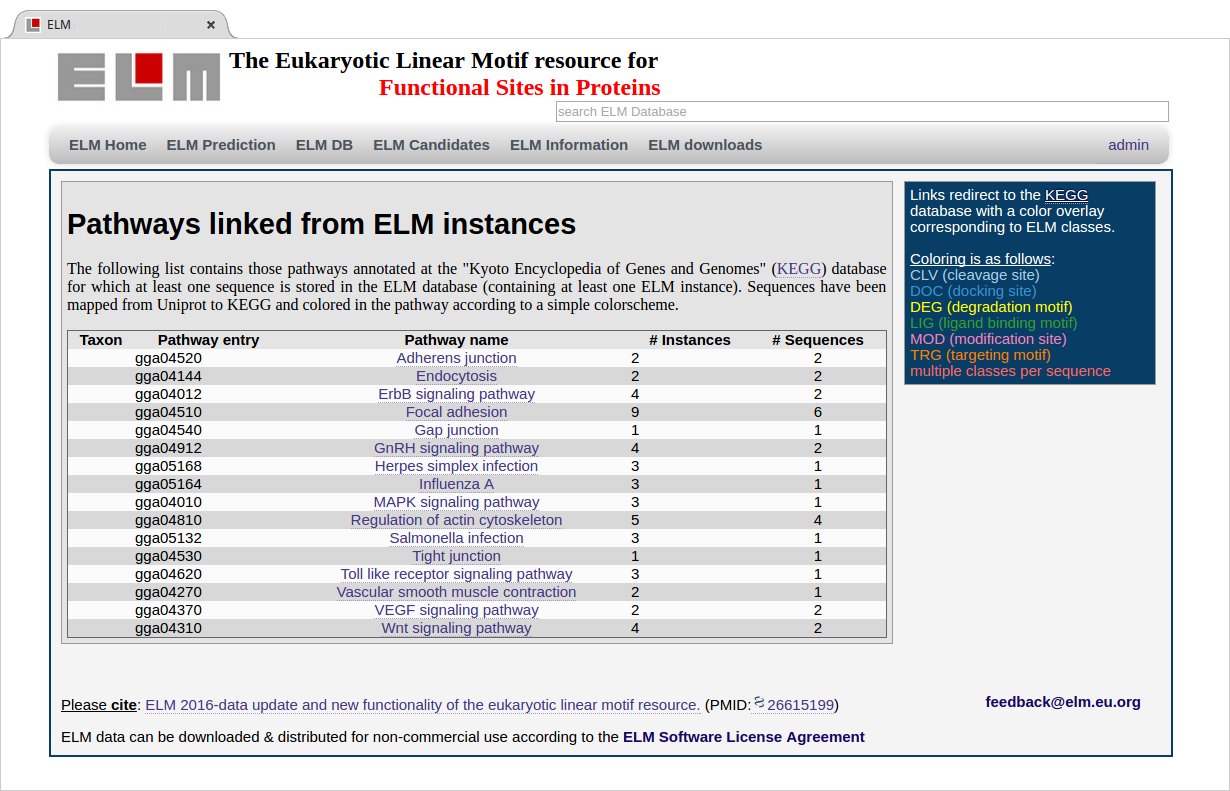
\includegraphics[width=\textwidth]{Figures/explore_content/pathways_example.png}
	\caption{
		A list of all KEGG pathways for the taxon \textit{Gallus gallus} involving proteins annotated in ELM. Note that multiple
		instances from a single sequence can be annotated for one pathway. The color scheme on the right is used for coloring instances
		on the KEGG website (see Figure~\ref{fig:explore_content_pathways_kegg}).
	}
	\label{fig:explore_content_pathways_example}
\end{figure}

\item On the ``ELM pathways'' page
	(Figure~\ref{fig:explore_content_pathways_example})
	click on the link \button{Gallus gallus} to navigate to the page
	containing all pathways annotated for
	chicken.

\begin{figure}[h!]
	\centering
	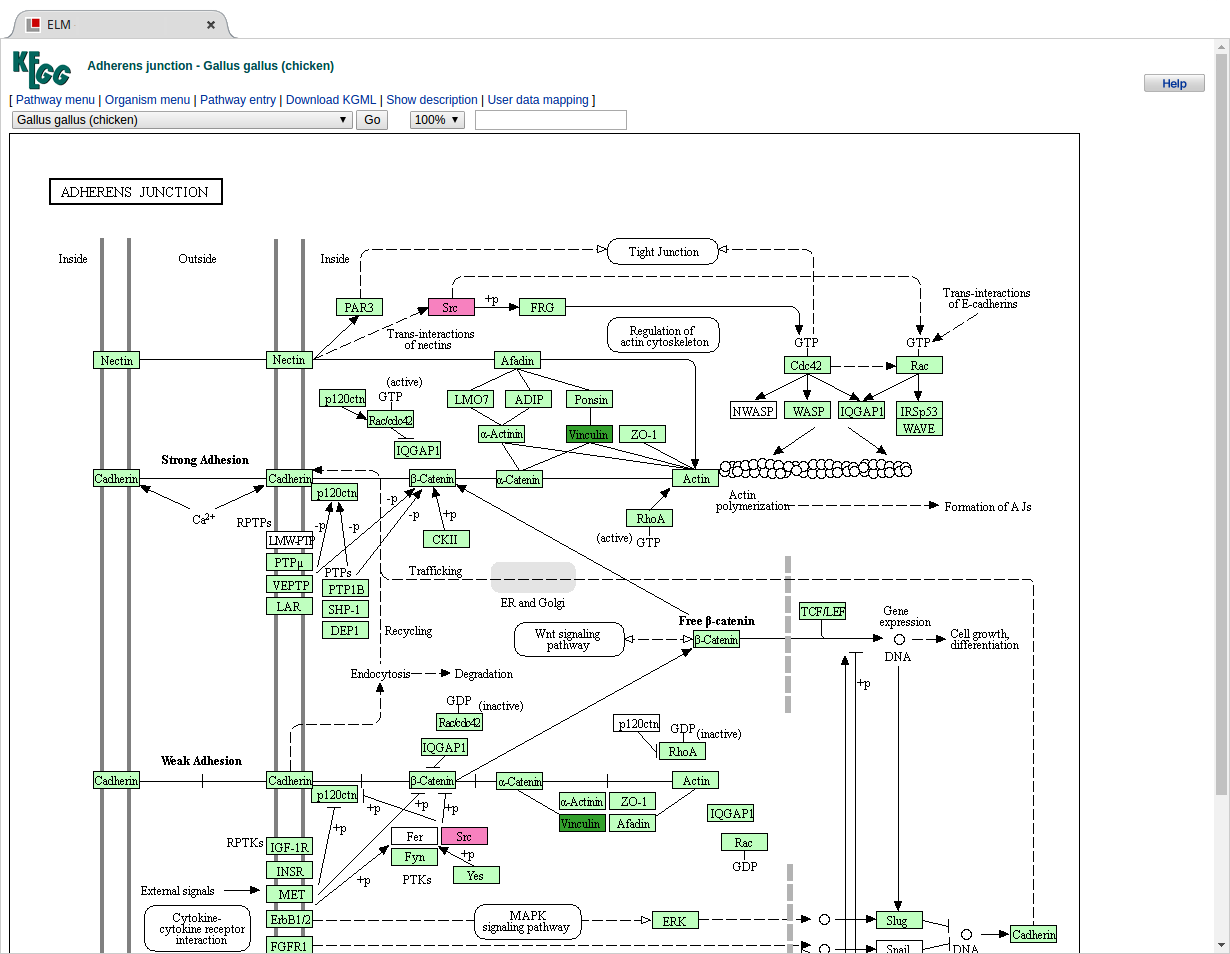
\includegraphics[width=\textwidth]{Figures/explore_content/pathways_kegg.png}
	\caption{
	An overlay of ELM annotations of proteins in the Adherens junction pathway in \textit{Gallus gallus}. The coloring of genes/proteins is as follows:
light blue=\motif{CLV} (cleavage site),
dark blue=\motif{DOC} (docking site),
yellow=\motif{DEG} (degradation motif),
green=\motif{LIG} (ligand binding motif),
pink=\motif{MOD} (modification site),
orange=\motif{TRG} (targeting motif),
red=multiple classes per sequence.
Light green boxes are colored by KEGG and represent the KEGG hyperlinks to GENES entries
    %, indicating the presence of genes in the genome and also the completeness of the pathway
    (see KEGG help \url{http://www.kegg.jp/kegg/document/help_pathway.html}).
	}
	\label{fig:explore_content_pathways_kegg}
\end{figure}

\item On the page with pathways annotated for chicken
	(Figure~\ref{fig:explore_content_pathways_example}),
	click on \button{Adherens junction} to the KEGG entry for this pathway,
	with each protein's color corresponding to ELM classes (see the color
	legend right side of Figure~\ref{fig:explore_content_pathways_kegg}).

%
% Subsection: Infections and Diseases
%
\subsection*{Browsing Infections and Diseases}
\label{subsec:explore_content_infections_and_diseases}

\begin{figure}[h!]
	\centering
	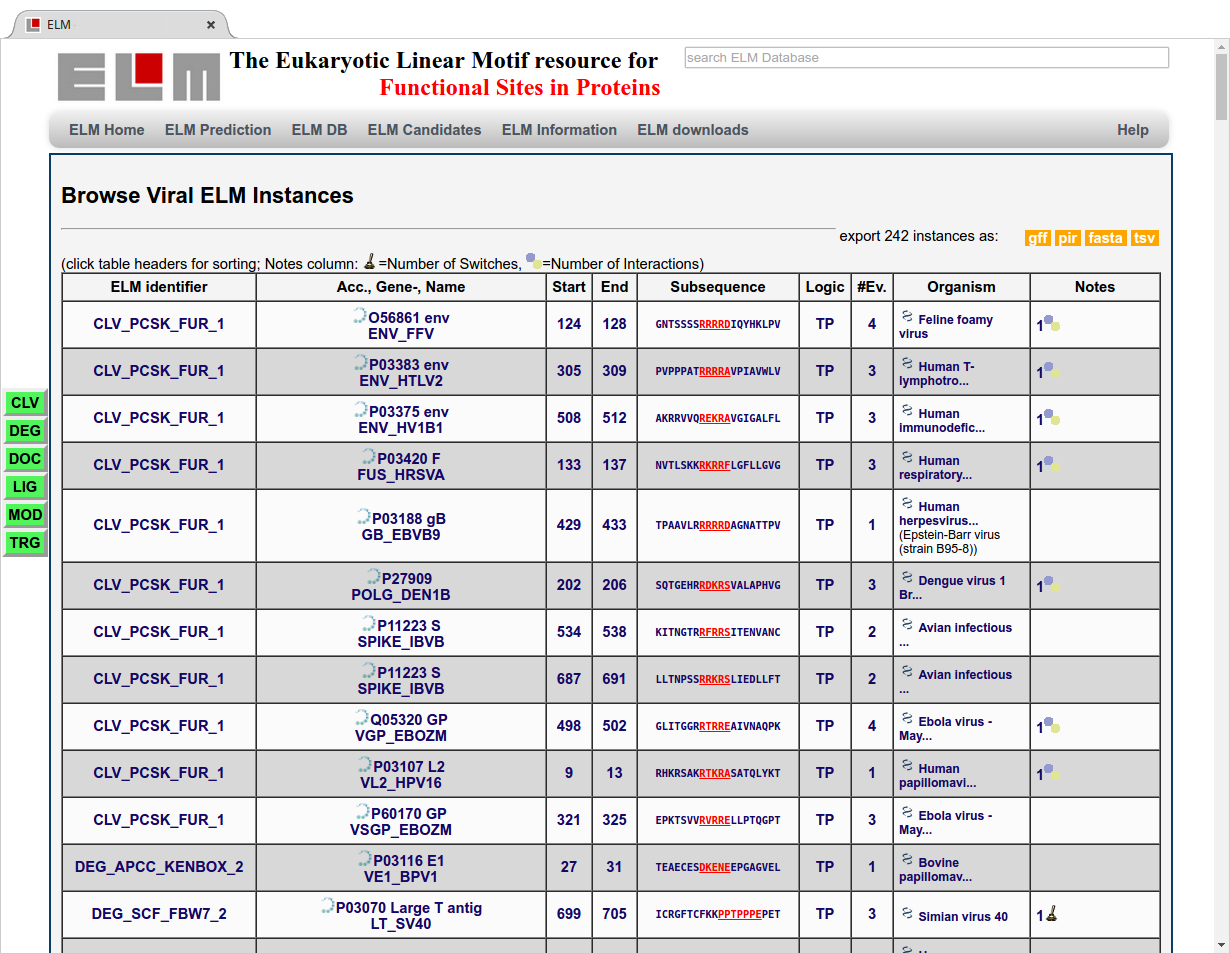
\includegraphics[width=\textwidth]{Figures/explore_content/viruses.png}
	\caption{
		A table of the ELM instances abused by viruses.
	}
	\label{fig:explore_content_viruses}
\end{figure}

\item \label{sec:explore_content_viruses} Click on the sub-menu \button{ELM virus instances} under \button{ELM DB}
	to see a list of all instances in ELM that have been annotated as being
	abused by viruses (Figure~\ref{fig:explore_content_viruses}).
	(The columns are identical to those listed in
	step~\ref{sec:explore_content_instances}, see Figure~\ref{fig:explore_content_instances}).

	\sdesc{The green buttons on the left can be used to filter this table
		by motif class. Click on the yellow links on the top right of
		the page to download the (complete) table in \fileformat{GFF},
		\fileformat{PIR}, \fileformat{FASTA} or \fileformat{TSV}
		format.}

\begin{figure}[h!]
	\centering
	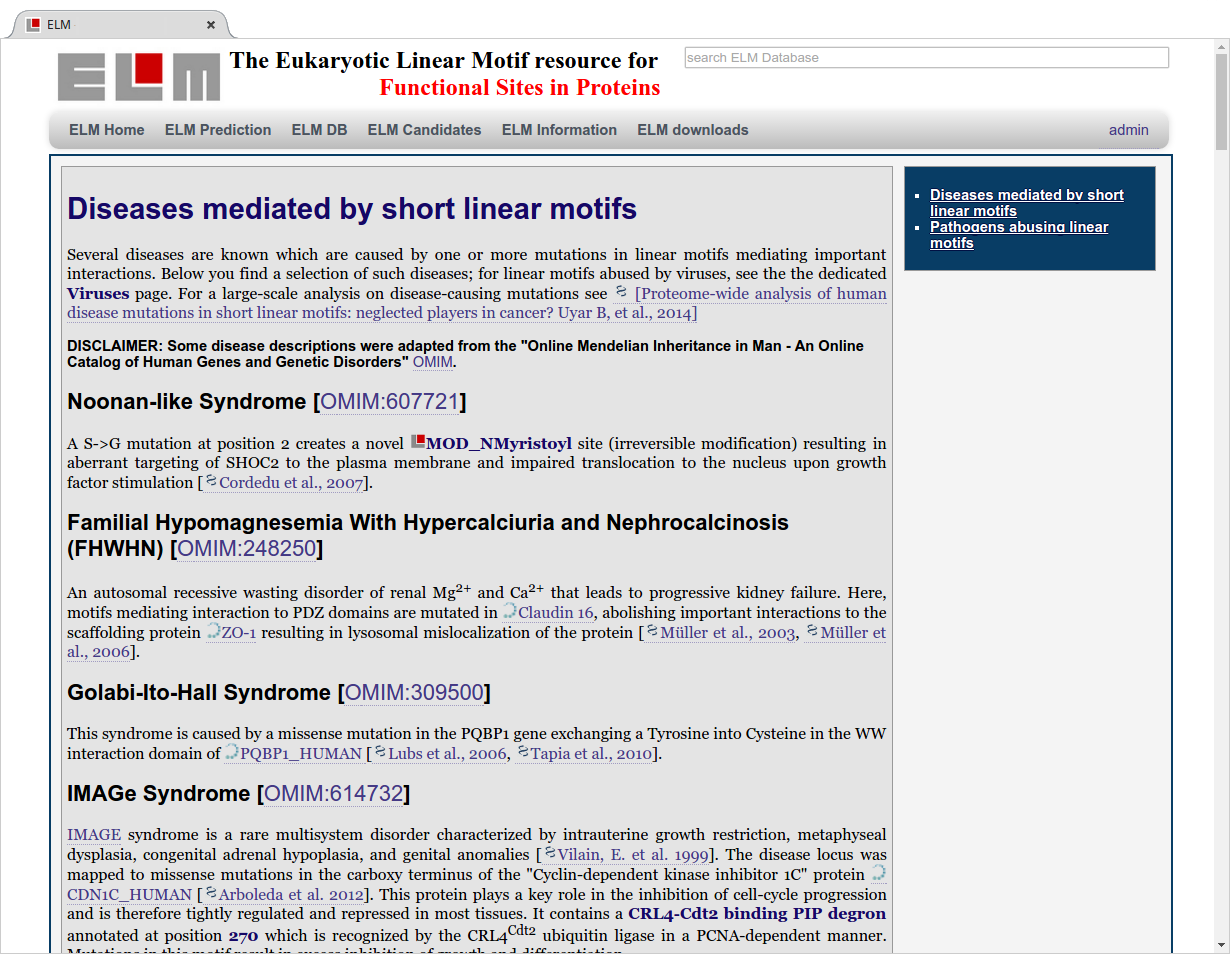
\includegraphics[width=\textwidth]{Figures/explore_content/diseases.png}
	\caption{
	A list of diseases that are mediated by short linear motifs. Disease description has been adapted from
	the ``Online Mendelian Inheritance in Man`` (OMIM) database \citep{17357067} and enriched with information about
	the role of the motif.
	}
	\label{fig:explore_content_diseases}
\end{figure}

\item Click on the sub-menu \button{ELM diseases} under \button{ELM DB} to see
	a list of diseases which are mediated by short linear motifs accompanied by
	a short description of the disease as well as the role of the motif.
	(Figure~\ref{fig:explore_content_diseases}). Disease information is taken
	from the ``Online Mendelian Inheritance in Man`` (OMIM) database
	\citep{17357067}.

%
% Subsection: Help page
%
\subsection*{Finding Help and Frequently Asked Questions}
\label{subsec:explore_content_help}

\begin{figure}[h!]
	\centering
	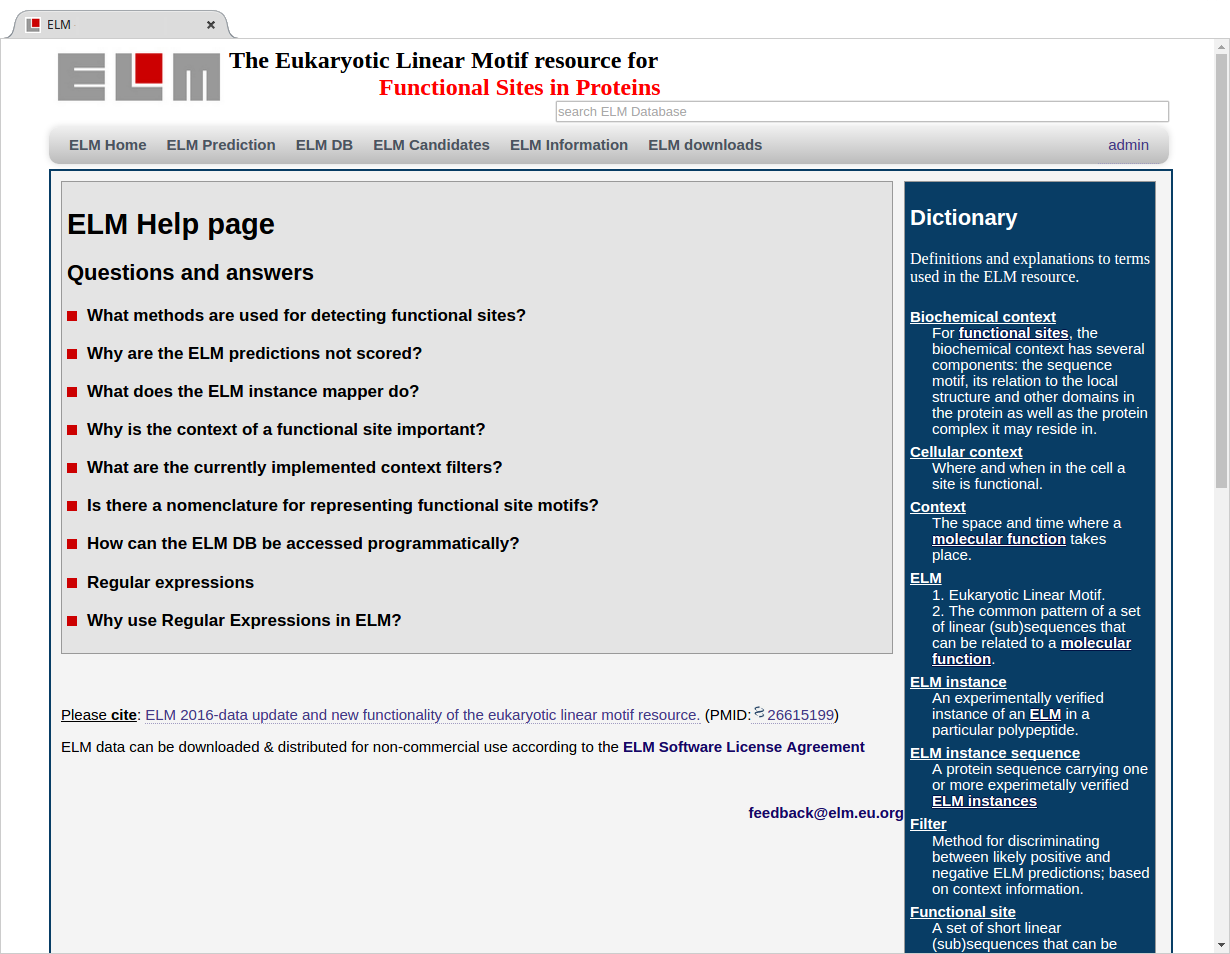
\includegraphics[width=\textwidth]{Figures/explore_content/help.png}
	\caption{
		The ELM ``Help'' and ``Questions \& Answers'' page.
		Users are encouraged to contact the authors via email if their questions
		regarding the ELM database can not be answered by this page.
	}
	\label{fig:explore_content_help}
\end{figure}

\item Click on the \button{Help} button on the right of the top navigation menu
	to visit the ELM Help page. This page has answers to the most
	Frequently asked questions, which you can see by clicking on a
	particular question. For example: Click on ``Regular expressions'' for
	a detailed description of the symbols used to build regular expressions
	to define motif classes.
\end{enumerate}


%%% General Search
\section{Exploring the Content of the ELM Database Using the General Search}
\label{sec:general_search}

A general search text box is available to query the entire collection of
manually curated information in the ELM database. This search field can be found in the header
of the ELM database website (see for example Fig.
\ref{fig:general_search_TP53_instances}). This search peforms a full-text
query across multiple selected data sources in the ELM database, including
ELM classes, instances, candidates, and switches. Using this general search is helpful in
getting information about a particular protein and its annotation status in the ELM database
(eg. full instance vs. candidate).

%
% Subsection: Necessary Resources
%
\subsection*{Necessary Resources}
\subsubsection*{Software \& Hardware}
A modern browser such as Firefox, Chrome, or Safari. ELM is best viewed
on a laptop or desktop computer, although tablets and smartphones will
also work.


%
% Subsection: General search
%
\subsection*{Using the General Search}
\label{subsec:general_search_using}
A modern browser such as Firefox, Chrome, or Safari. ELM is best viewed
on a laptop or desktop computer, although tablets and smartphones will
also work.


\begin{enumerate}

\begin{figure}[h!]
	\centering
	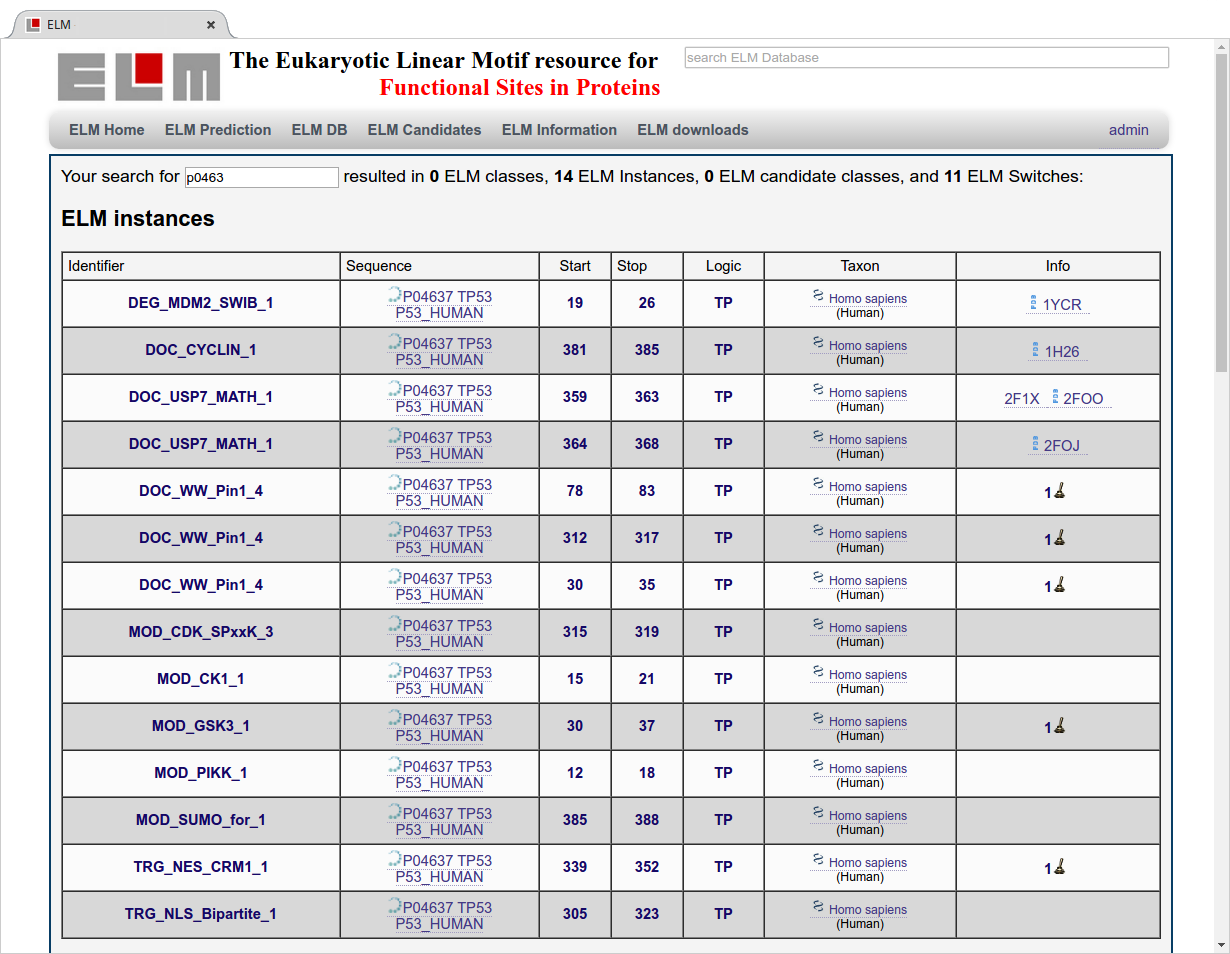
\includegraphics[width=\textwidth]{Figures/general_search/P04637_instances.png}
	\caption{
		The instances retrieved when performing a general search for
		\uniprot{P53\_HUMAN} using its UniProt identifier ``P04637''.
	}
	\label{fig:general_search_P04637_instances}
\end{figure}

\begin{figure}[h!]
	\centering
	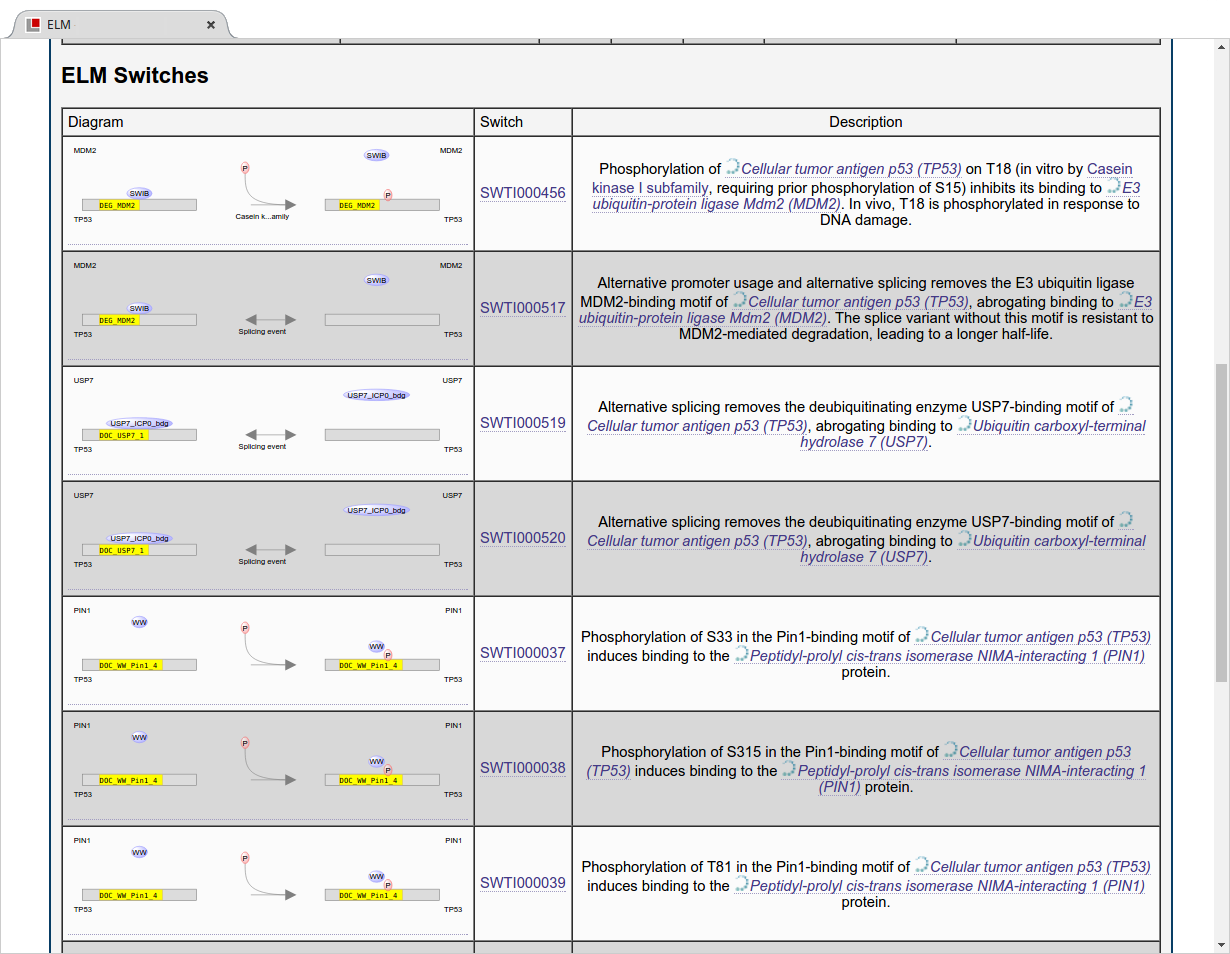
\includegraphics[width=\textwidth]{Figures/general_search/P04637_switches.png}
	\caption{
		The switches found when performing a general search for
		\uniprot{P53\_HUMAN} using its UniProt identifier ``P04637'',
	}
	\label{fig:general_search_P04637_switches}
\end{figure}


\item Use the general search field (on the top of the page) to do a general
	search for p53 using its UniProt identifier by typing ``P04637'' in the
	search field and hitting ``Enter''. This will perform a query
	across multiple tables of the ELM database to find any matches to the
	search query ``P04637''.
	In this case, the results are grouped into matching instances
	(Figure~\ref{fig:general_search_P04637_instances})
	candidate classes and switches
	(Figure~\ref{fig:general_search_P04637_switches}).
	As there are no classes with ``P04637'' in the name or description, no classes are
	returned for this section of the query.

% TODO: describe candidate classes (&instances) better
	\sdesc{
		The ``candidate classes'' are a collection of putative future ELM classes, which are not yet fully annotated, often submitted by
		ELM users. Keep in mind that these are a first draft on ELM classes and are still pending curation.
	}

\begin{figure}[h!]
	\centering
	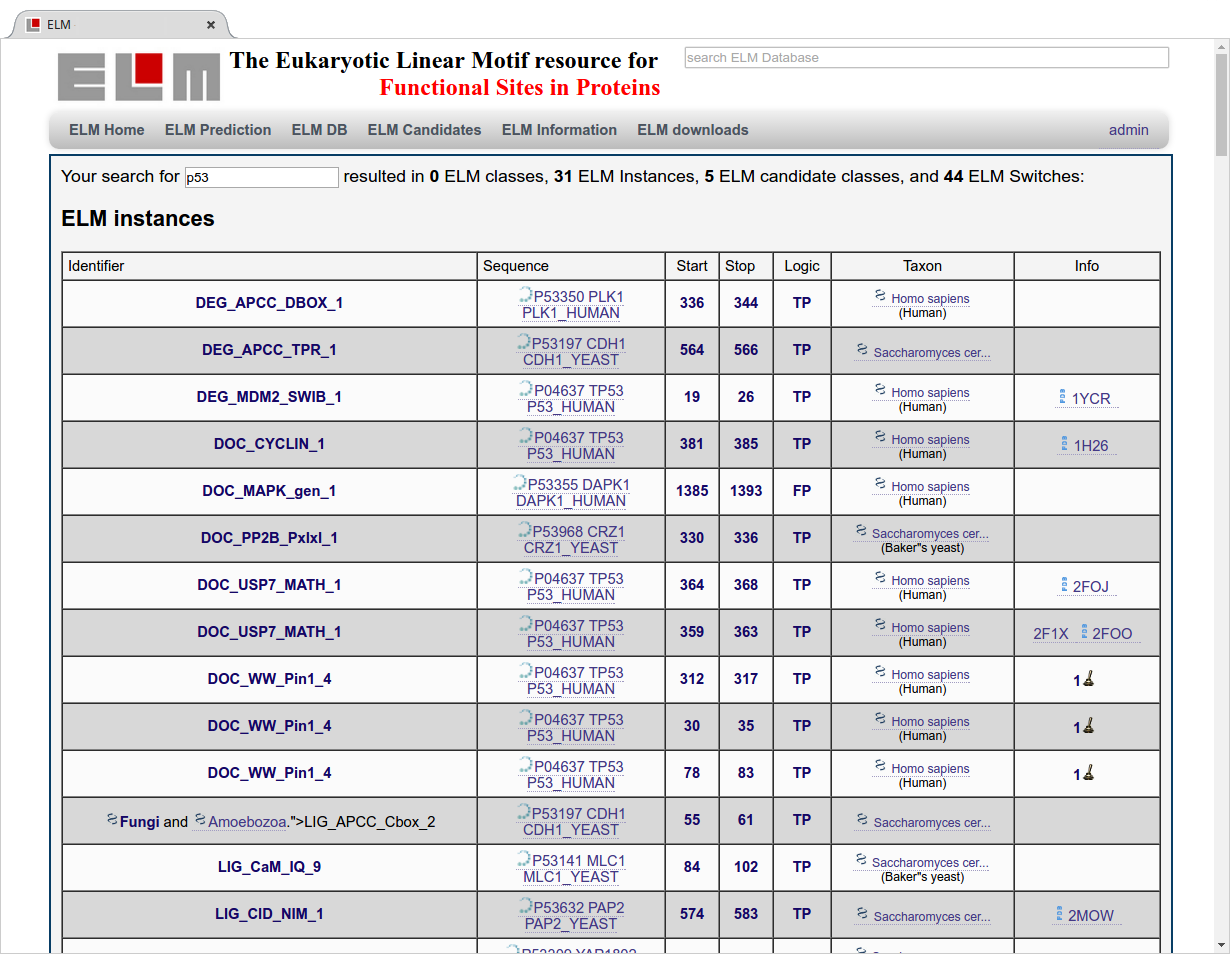
\includegraphics[width=\textwidth]{Figures/general_search/TP53_instances.png}
	\caption{
		The results retrieved when performing a general search for
		\uniprot{P53\_HUMAN} using the query ``p53''.
	}
	\label{fig:general_search_TP53_instances}
\end{figure}

\item Perform a search using the keyword ``p53'' in the general search field
	instead of its UniProt identifier ``P04637''.
	The set of results retrieved using this term as the search query
	(Figure~\ref{fig:general_search_TP53_instances})
	are different, returning 31 instances and 44
	switches (instead of 14 and 11). The reason for this is that the
% TODO: HD: maybe discuss this rather in the commentary section?
% Marc: I'm OK with this here. This is very relevant to the 'general search' only - Marc
	phrase ``p53'' also matches the UniProt identifier of
	\uniprot{CDH1\_YEAST} (P53197). This is probably not what you had in mind when using this search term, so it is important to keep in mind
	to check for such false positive search results, when searching the database.

\end{enumerate}

\clearpage

%%% P53
\section{Detecting Short Linear Motifs in Protein Sequences}
\label{sec:predicting_p53}

One of the most useful (and used) features in ELM is the ability to
detect motifs in proteins and sequences. Given a protein's amino acid
sequence, the ``ELM Predictions'' pipeline searches for occurrences of
each motif class using regular expressions, applies a set of filters to
remove false positives and creates a diagram to visualize resulting
set of putative motifs.

In this protocol we will be viewing the manually annotated data of a
typical protein, using p53 (UniProt ID: \uniprot{P53\_HUMAN}/P04637) as an
example. We will cover how to find the manually annotated motifs and instances,
the references used to annotate each
instance, the experimental protocols used, and additional information including
relationships to biological pathways (KEGG), diseases (OMIM) and molecular
switches (switches.ELM).

%
% Subsection: Necessary Resources
%
\subsection*{Necessary Resources}
\subsubsection*{Software \& Hardware}
A modern browser such as Firefox, Chrome, or Safari. ELM is best viewed
on a laptop or desktop computer, although tablets and smartphones will
also work.


\begin{enumerate}

%
% Subsection:Predicting ELM instances
%

\subsection*{Predicting ELM instances: Input form}
\label{subsec:predicting_p53_input}

\begin{figure}[h!]
	\centering
	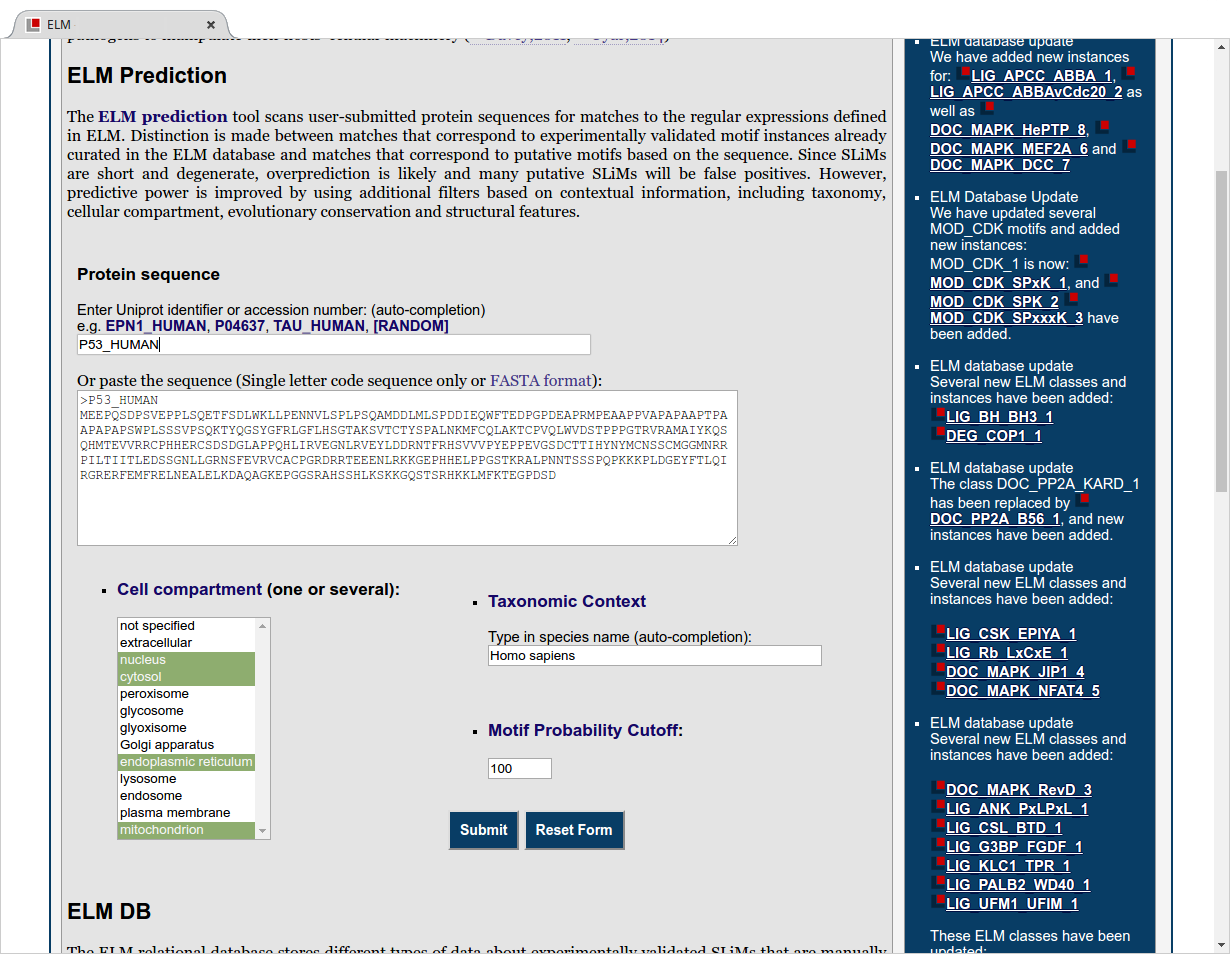
\includegraphics[width=\textwidth]{Figures/predicting_p53/elm_search.png}
	\caption{
	The ELM input page for predicting motifs in a protein. Here, all fields have been filled in; strictly only the protein ID field is
	necessary to perform a search.
	}
	\label{fig:predicting_p53_elm_search}
\end{figure}

\item Open a browser, and navigate to the ELM homepage: \url{http://elm.eu.org}.\label{sec:predicting_p53_elm_search}
	Enter the UniProt ID \uniprot{P53\_HUMAN} in the search field labelled
	``Enter a UniProt identifier or accession number''. While typing, the page should
	autocomplete your input ``\uniprot{P53\_HUMAN} / P04637 (\textit{Homo
	sapiens})'' and already pre-fill other fields of the input form (Figure~\ref{fig:predicting_p53_elm_search}).
	Click on this entry to confirm that you want to search for
	motifs in this protein. Click on \button{Submit} to send the query to
	the server.

	\sdesc{The autocompletion mechanism queries UniProt for the given protein
		identifier; if it succeeds, then additional information from
		UniProt will be used to auto-populate the input boxes. In this
		example, \uniprot{P53\_HUMAN} is recognized as a human protein,
		and so ``Homo sapiens'' is automatically filled in the
		``Taxonomic Context'' field. Also, p53 has been annotated (by
		UniProt) to be localized to nucleus, cytosol, endoplasmic
		reticulum and mitochondrion, so these are also automatically
		applied as search criteria. The motif cutoff of ``100'' is a
		sufficiently high (lenient) threshold to ensure no motif class
		is filtered out based on motif probability.}

\item Select the search criteria (optional). 
%	It is possible to limit the results by ``Cell compartment'', ``Taxonomic Context'' or by changing the ``Motif Probability Cutoff''.
	To restrict the search to include
	motifs that are active only in certain cellular compartments, select one or
	more from the ``Cell compartment'' list (use the ``control'' key to select more than one
	option). It is also possible to select a ``Taxonomic Context'' to
	restrict the search to motifs from certain species. Start typing a
	species name in the ``Taxonomic Context'' input field to get an
	auto-completed list of species to select from. Additionally, a ``Motif
	probability cutoff'' can be used to only retain ELM classes whose
	pattern probability is below the given value.
	These filters are implemented later in \ref{sec:predictions_cv_0974}).
	For now, leave all all filters at the default values that were
	auto-populated for p53. 


%TODO: HD add probability filter to commentary

TODO: Repeat search using stringent filters (homo sapiens, nucleus, 0.01) Do we want to do this? - Marc

YES, we do. HD
%	At the moment, step 1. & 2. are confusing as the second 'overwrites' the
%	first. better to continue with 3 (as 2) and repeat 2 later with
%	different settings
%
% Marc: Sorry, my mistake. I had intended to make this protocol use default
% values, and Hugo's procol to use filters. I've adapted the existing text to
% reflect this.

%
% Subsection: Understanding results: graphical summary
%

\subsection*{Interpreting the prediction results: Graphical Summary}
\label{sec:predicting_p53_graphical_summary}

\item \label{sec:predicting_p53_submit} Click \button{submit} to start searching for motifs. You will be brought
	to an intermediate page indicating that your results are being
	processed, and should be redirected to the final results page
	within a minute. You can bookmark this page: The results are stored for
	a week.

	\sdesc{The Results are summarized in the first figure on the results
		page (see Figure~\ref{fig:predicting_p53_results_summary}).
		The graphical summary shows the
		results generated by the ELM prediction pipeline, combined with
		additional filters and information from external resources. The
		visualization should help you interpreting the results and to
		assess whether or not a motif is present in a sequence, as well
		as how likely it is to be functional based on its structural
		context and evolutionary conservation. Motif instances that
		are manually annotated in the database appear as red (TP) or
		yellow (FP) ovals in the graphic. Blue/gray squares represent
		predicted motif occurrences.}

\begin{figure}[h!]
	\centering
	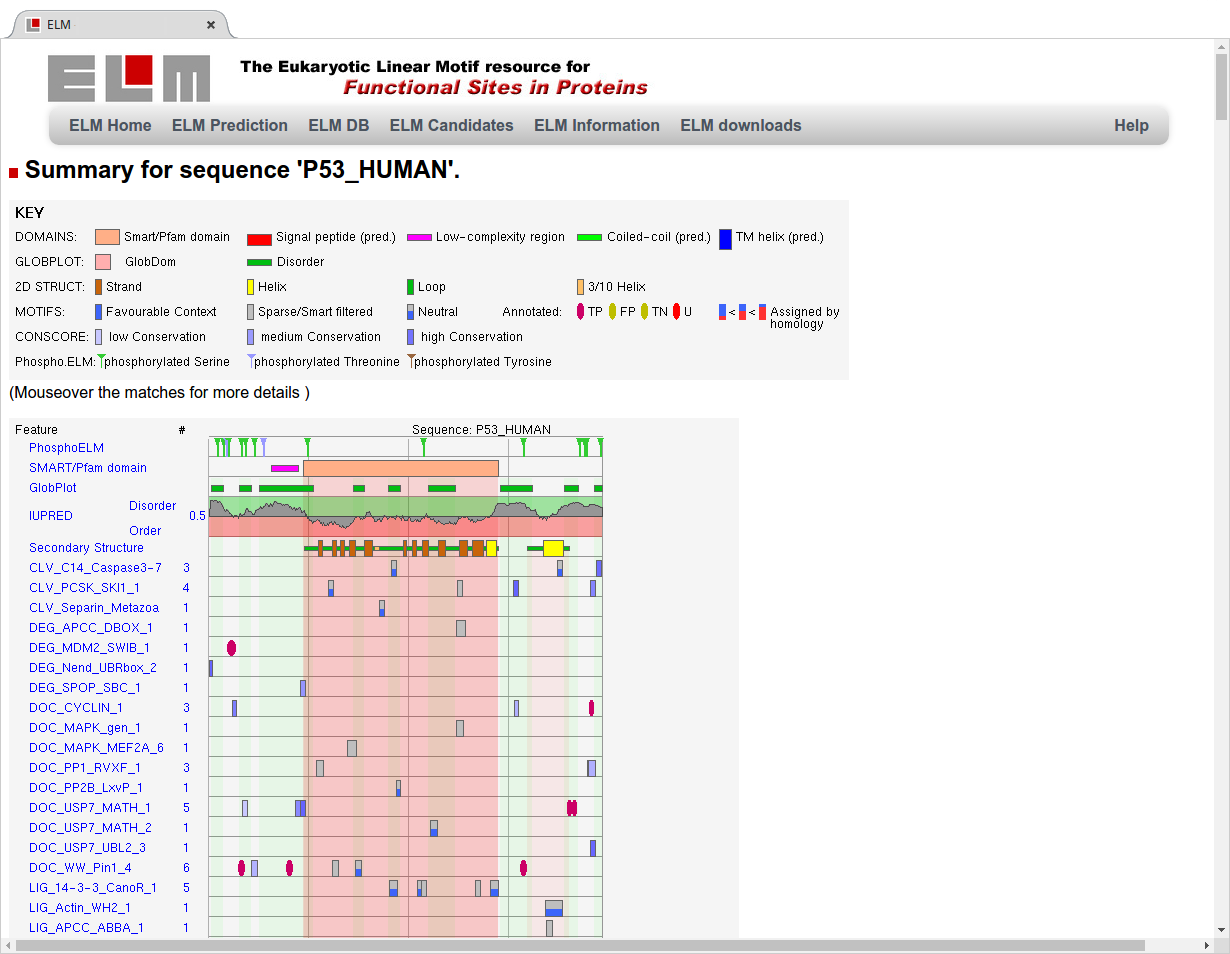
\includegraphics[width=\textwidth]{Figures/predicting_p53/elm_results_summary.png}
	\caption{
	The graphical results summary of the ELM Prediction pipeline for
	\uniprot{P53\_HUMAN}. Note that not all motif detections are shown (the
	image is truncated at the bottom). The top five rows show a set of
	structural features. Annotated and predicted motifs are shown as
	differently colored ovals/boxes. The info screens for three motifs are
	shown: \motif{CLV\_C14\_Caspase3-7}, \motif{DEG\_MDM2\_SWIG\_1} and
	\motif{CLV\_Separin\_Metazoa}.
	}
	\label{fig:predicting_p53_results_summary}
\end{figure}

\item \label{sec:predicting_p53_results_phosphorylation} The first row contains phosphorylation sites as retrieved from
	phospho.ELM \citep{21062810}, and whether the phosphorylated amino
	acid is a serine, threonine or tyrosine. Phospho.ELM is a database of
	manually annotated phosphorylation sites obtained from scientific
	publications from low and high-throughput experiments. You can follow
	the link to phospho.ELM by clicking on the phosphorylation site in the
	image to get more information on individual phosphorylation sites.

	\sdesc{Phosphorylation sites are only available when the search is
		performed with a protein accession (eg. \emph{not} with a FASTA
		sequence alone) in step \ref{sec:predicting_p53_elm_search} and there is relevant information
		annotated in the phospho.ELM database. Phosphorylation sites
		are relevant to interpret ELM motif predictions when the
		predicted motif requires to be phosphorylated (as in several
		docking and ligand binding motifs) and for predicting
		phosphorylation motifs.}

\item The second row shows SMART and Pfam domains detected by the SMART
	database \citep{9600884, 25300481, 9600884}
	(Figure~\ref{fig:predicting_p53_results_summary}). Hover the
	mouse over these domains to see their names and exact start and end
	positions.

	\sdesc{ In order to be functional motifs to be accessible, and
		therefore they are usually not found within globular domains
		and structured regions \citep{21909575}. Any motifs detected
		by the ELM prediction pipeline inside of a smart domain are
		less likely to be functional, and are shown as a gray box
		background (see commentary section "Structure Filter" at page \pageref{StructureFilter}). }

\item The third row shows globular and disordered regions in the
	sequence as predicted by GlobPlot \citep{12824398}. The fourth
	and fifth rows
	contain results from IUPred \citep{15955779}, another
	predictor of disordered protein regions. Protein segments with
	an IUPred score above 0.5 are considered to be disordered 
	(see commentary section "Disorder Filter" at page \pageref{DisorderFilter}).

	\sdesc{Motifs are typically only functional when found in intrinsically
		disordered regions. Any motif occurrence detected by the ELM
		prediction pipeline that falls within disordered regions are
		more likely to be functional.}

\item The 5th row (Figure~\ref{fig:predicting_p53_results_summary}) contains
	information on the protein's structure (see commentary section "Structure Filter" at page \pageref{StructureFilter}). The secondary structure is
	predicted using a pipeline mapping motif occurrence onto high quality
	reference domain structures \citep{19852836}. Check the graphical
	representation, and if the output of the secondary structure filter and
	the disorder predictors agree with respect to which parts of the
	sequence are considered structured and which are disordered.

\item The remainder of the figure (below ``secondary structure'' output)
	displays predicted and annotated motif instances, overlayed with the
	structural context from rows 2 and 3 (SMART domains and GlobPlot). A
	blue square indicates a single motif occurrence, and intensity of the
	color indicates the conservation of this sequence across a group of in
	homologous proteins.
	Boxes in gray are motif occurrences that have been filtered out by the
	structure filter. Boxes that are blue \& gray are neutral (
	residing in structural context, but the secondary structure detected a
	loop region). If the sequence is already present in the ELM database,
	any motif instances that have already been annotated are shown as
	ovals. Lastly, any motifs detected which are annotated to be
	functional in homologous sequences, are shown as red \& blue
	rectangles.

	\sdesc{ In the case that not enough homologous sequences were detected
		to build an alignment, no conservation score can be calculated.
		Therefore all of the motif occurrences will be shown in a
		uniform shade of blue. }

\item Place the cursor over the blue box for motif occurrence
	\motif{CLV\_C14\_Caspase3-7} at the end of the sequence (
	position 388--392). This will trigger the green and yellow
	information screen shown on the top right in Fig.
	\ref{fig:predicting_p53_results_summary}.
	This motif is in a disordered region, and has not been
	filtered out by the structural filter. Also, its conservation score
	of 0.910 is very high, indicating that this motif is highly conserved.

	\sdesc{The confidence score is based on how conserved the sequence is
		across a set of homologous proteins from other sequences.
		The higher the conservation score (max. 1.0), the more conserved
		the motif's sequence is, and the more likely it is a functional
		motif for this prediction
		(see commentary section "Conservation Filter" at page \pageref{ConservationFilter}).}

\item \label{sec:predicting_p53_results_structure_filter} Place the cursor over the blue \& gray rectangle for motif
	\motif{CLV\_Separin\_Metazoa} at position 171--175, a motif
	which was flagged as ``neutral'' by the ELM prediction pipeline.
	This will trigger the information screen (with the pink header) shown
	in Figure~\ref{fig:predicting_p53_results_summary} to appear.
	This motif resides inside of the p53 Pfam domain, and thus has been
	subjected to ``structural filtering''. However, the secondary structure
	prediction suggests this motif occurs within the looped region of this
	domain, so may be accessible.

	\sdesc{The information screen pop-up
	shows scores for all of the individual criteria used by the secondary
	structure filter: The name of the domain, the \emph{accessibility
	score} , \emph{secondary structure score}, \emph{combined total score},
	and the associated \emph{total score P-value} \citep{19852836}.}

\item Place the cursor over the red oval for \motif{DEG\_MDM2\_SWIG\_1} at
	position 19--26. This motif is an annotated instances in the
	ELM database, and is therefore a bona-fide experimentally validated
	instance.

%TODO: Marc: a little more description here?

\begin{figure}[h!]
	\centering
	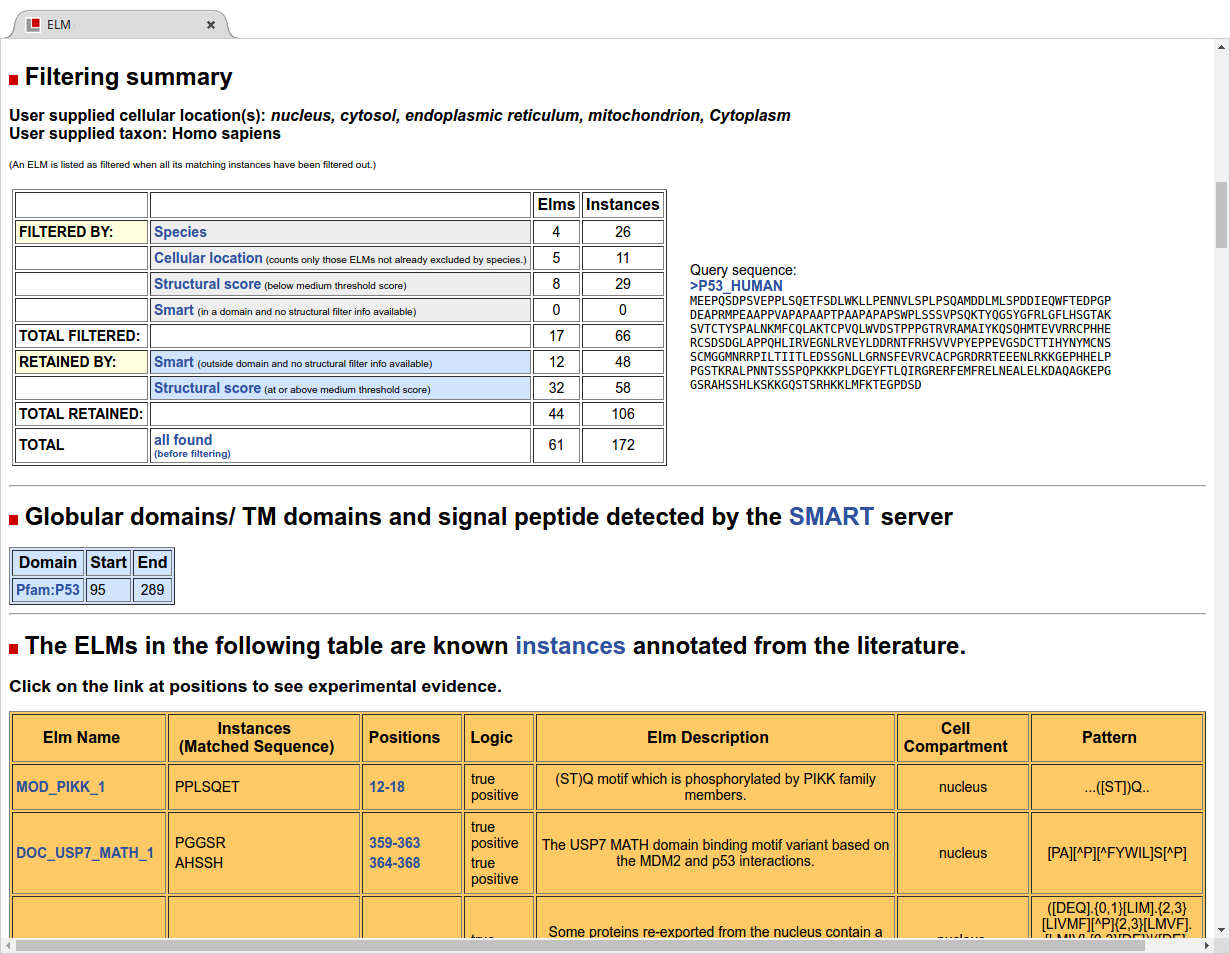
\includegraphics[width=\textwidth]{Figures/predicting_p53/elm_results_alignments_filtering_domains.png}
	\caption{
	This section of the results contains additional details on the
	homologue alignments used to calculate the conservation score,
	filtering results and globular domains.
	}
	\label{fig:predicting_p53_elm_results_alignment_filtering_domains}
\end{figure}

\item \label{sec:predicting_p53_results_alignment} Scroll down to below the results graphic to find additional information
	on the ELM prediction pipeline's results
	(Figure~\ref{fig:predicting_p53_elm_results_alignment_filtering_domains}).
	The first
	section contains links to download or view the multiple sequence
	alignments of homologous proteins used to calculate the conservation
	score. Click on the link ``Click here to enable the multiple sequence
	alignment viewer'' to open the alignment in Jalview (note: this
	requires the Java browser plugin, which might not be available on some
	browsers). Alternatively you can also download the ``alignment'',
	``conservation features'' and ``phosphosite features'' files separately
	to view on a desktop (non-browser) installation of Jalview
	\citep{19151095}.

	\sdesc{ The search for possible homologues is performed against the
		UniRef90 database, a dataset of protein sequences with less
		than 90 percent identity between any two of them
		\citep{17379688}. It may occur that the BLAST results
		are not finished when the results page is shown: We suggest to
		refresh the page if you see the message ``Either not enough
		data available to calculate a sequence alignment or the
		calculations haven't finished yet''. In some cases it is also
		possible that no homologues will be detected. If you have
		refreshed the page after waiting for more than 3 minutes, this
		is most likely the case.}

\item Scroll down to the section titled ``Filtering Summary'' to view some
	statistics about how many motifs and instances were filtered out
	(Fig.
	\ref{fig:predicting_p53_elm_results_alignment_filtering_domains}).
	The first two lines contain information on whether
	and which filters were applied in step \ref{sec:predicting_p53_elm_search} of this protocol.
	In this case 4 motifs representing 26 instances were filtered
	out as they did not occur in \textit{Homo sapiens}. An additional 5
	motifs (representing 11 instances) were filtered out because they are
	not annotated to the cell compartments automatically filled in on the
	search page (step \ref{sec:predicting_p53_elm_search}).
	The next three lines (``SMART'' \& ``Structural score'') show how many
	motifs and instances were not removed by the SMART and Secondary
	structure filters. A total of 42 motifs (representing 106 instances)
	passed the structural filter.

	\sdesc{Note that the graphical summary above does not contain sequences
		filtered out by the ``cell compartment'' and ``taxonomic
		context'' filters. However those filtered out by
		the SMART and Structural scores are shown in the graphic above
		(as gray rectangles).}

\begin{figure}[h!]
	\centering
	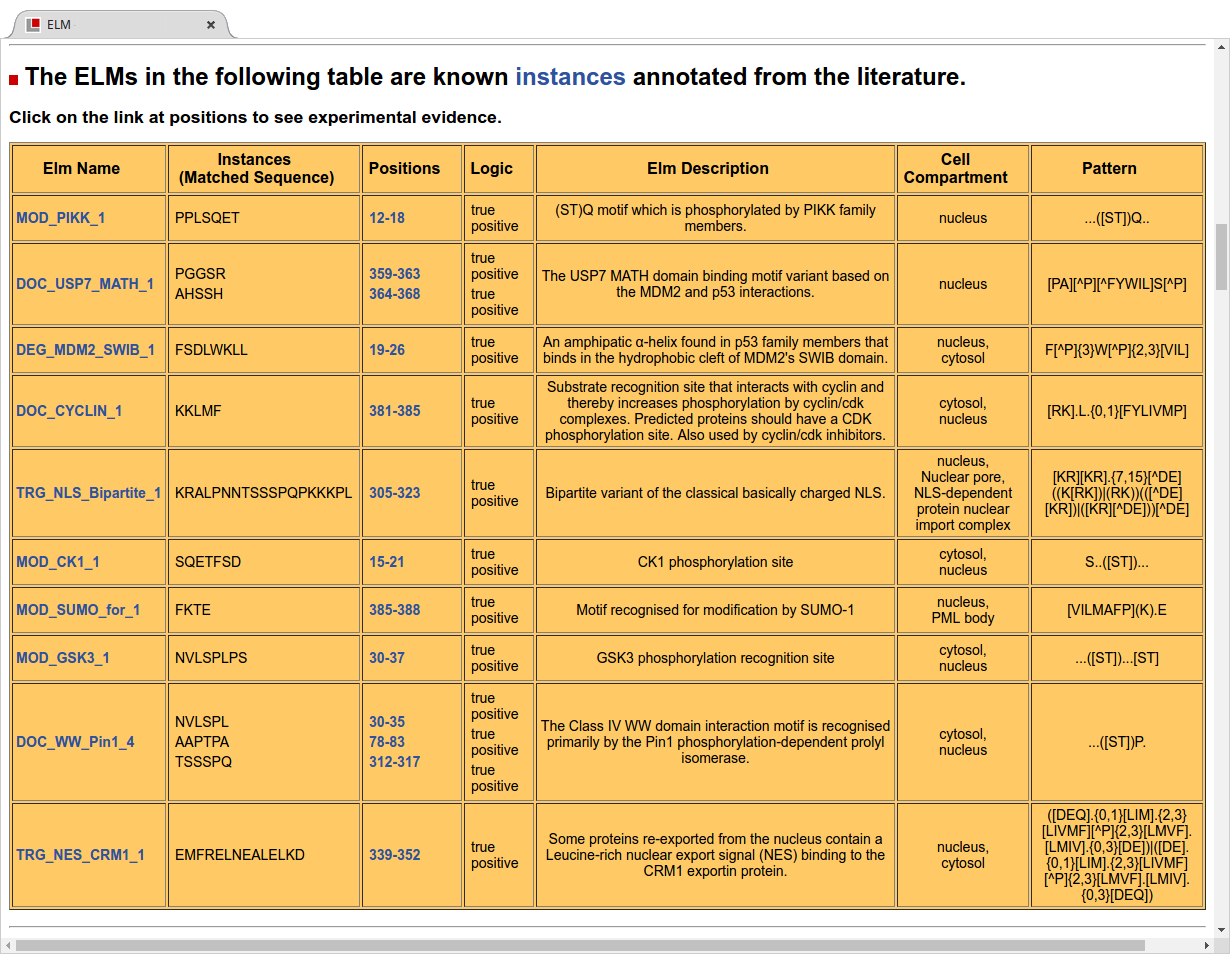
\includegraphics[width=\textwidth]{Figures/predicting_p53/elm_results_known.png}
	\caption{
		The ELM prediction pipeline section displaying the p53 motifs
		that are ``known'', and have been annotated in the ELM
		database.
	}
	\label{fig:predicting_p53_elm_results_known}
\end{figure}

\item Scroll down to the section with the header ``Globular domains/ TM domains
	and signal peptide detected by the SMART server''
	(Figure~\ref{fig:predicting_p53_elm_results_alignment_filtering_domains}).
	This section contains information on which domains were detected by the
	SMART server, and their positions. Clicking on their names will bring
	you to the entry for that domain on the SMART or Pfam homepage.
	In this case the only domains detected is the ``p53'' Pfam domain.

\item On the results page, scroll down to the heading: ``The ELMs in the
	following table are known instances annotated from the literature''
	(\ref{fig:predicting_p53_elm_results_known}).
	This table has details of the motifs and instances which have been
	manually annotated in the ELM database. The columns show each motif
	name, the sequence(s) that matched the motif as well as their starting
	and ending positions and the logic of the annotation followed by a
	short description of each motif, to which cell compartments its has
	been associated, and finally the regular expression of the motif.

\begin{figure}[h!]
	\centering
	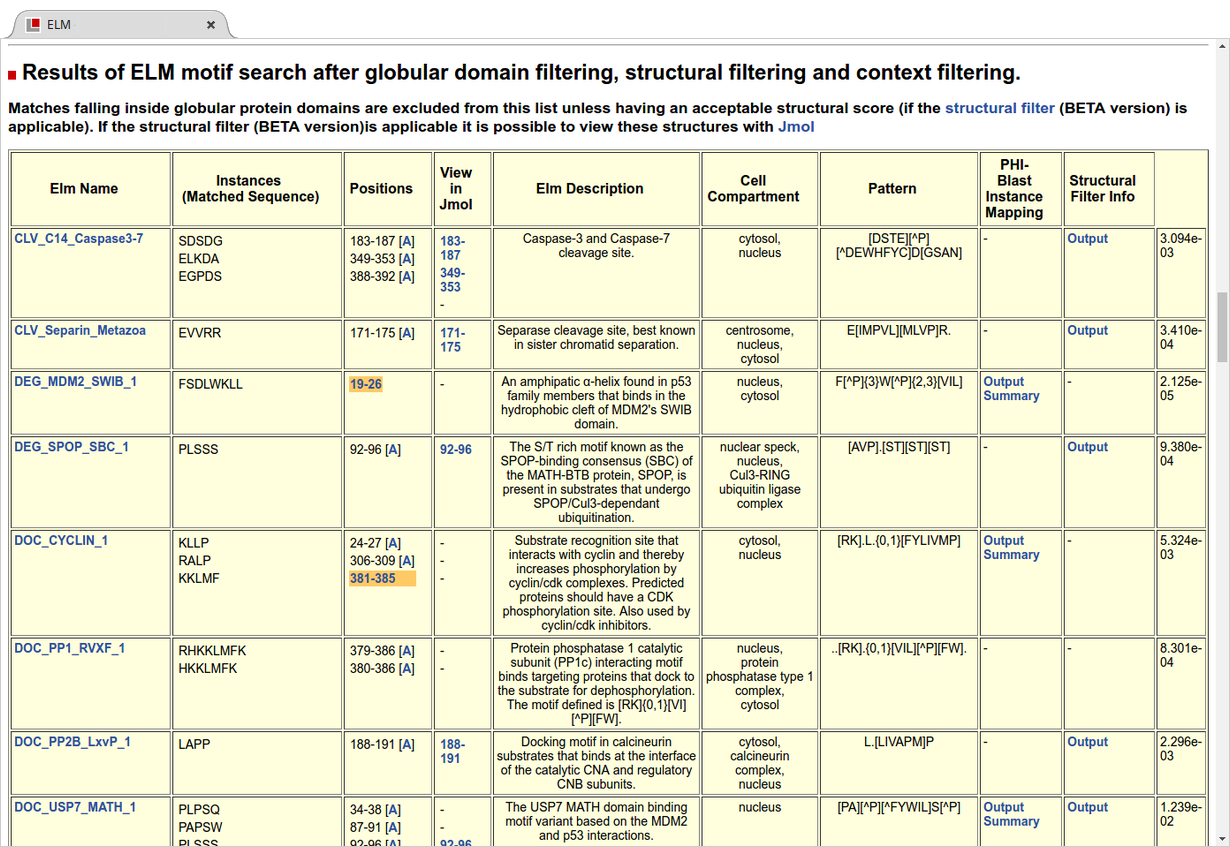
\includegraphics[width=\textwidth]{Figures/predicting_p53/elm_results_motifs.png}
	\caption{
	This table contains the list of putative motifs detected in the query sequence (only
	the top part of the table is shown). These are ``predictions`` in the sense
	that each of these motifs could be found in the sequence after applying (structure/context) filtering, however no experimental evidence has been annotated (yet) to determine if they are biologically functional.
	}
	\label{fig:predicting_p53_elm_results_motifs}
\end{figure}

\item Scroll further down to the section title ``Results of ELM motif search
	after globular domain filtering, structural filtering and context
	filtering'' to obtain an overview of all of the motifs and motif
	instances detected
	(\ref{fig:predicting_p53_elm_results_motifs})
	Each of the rows is a ``predicted'' motif: A sequence matching a
	motif's regular expression has been detected that has also passed the
	``structural filter''.
	Each row displays the motif identified, the matching peptide
	sequence and its position. Additional information is shown about the
	motif, its cell compartment and its regular expression. If the motif
	was detected in a homologue, the column ``PHI-Blast Instance
	mapping'' contains a link to the multiple sequence alignment of the
	homologous proteins. If a motif instance has been filtered out
	by the ``structural filter'', the ``Structural filter info'' column
	contains a link to a page with details on why.
	The last column contains information on the Probability filter: the
	probability reflects the chance to observe this motif in any random
	amino acid sequence (see section \ref{sec:explore_content})

\begin{figure}[h!]
\centering
	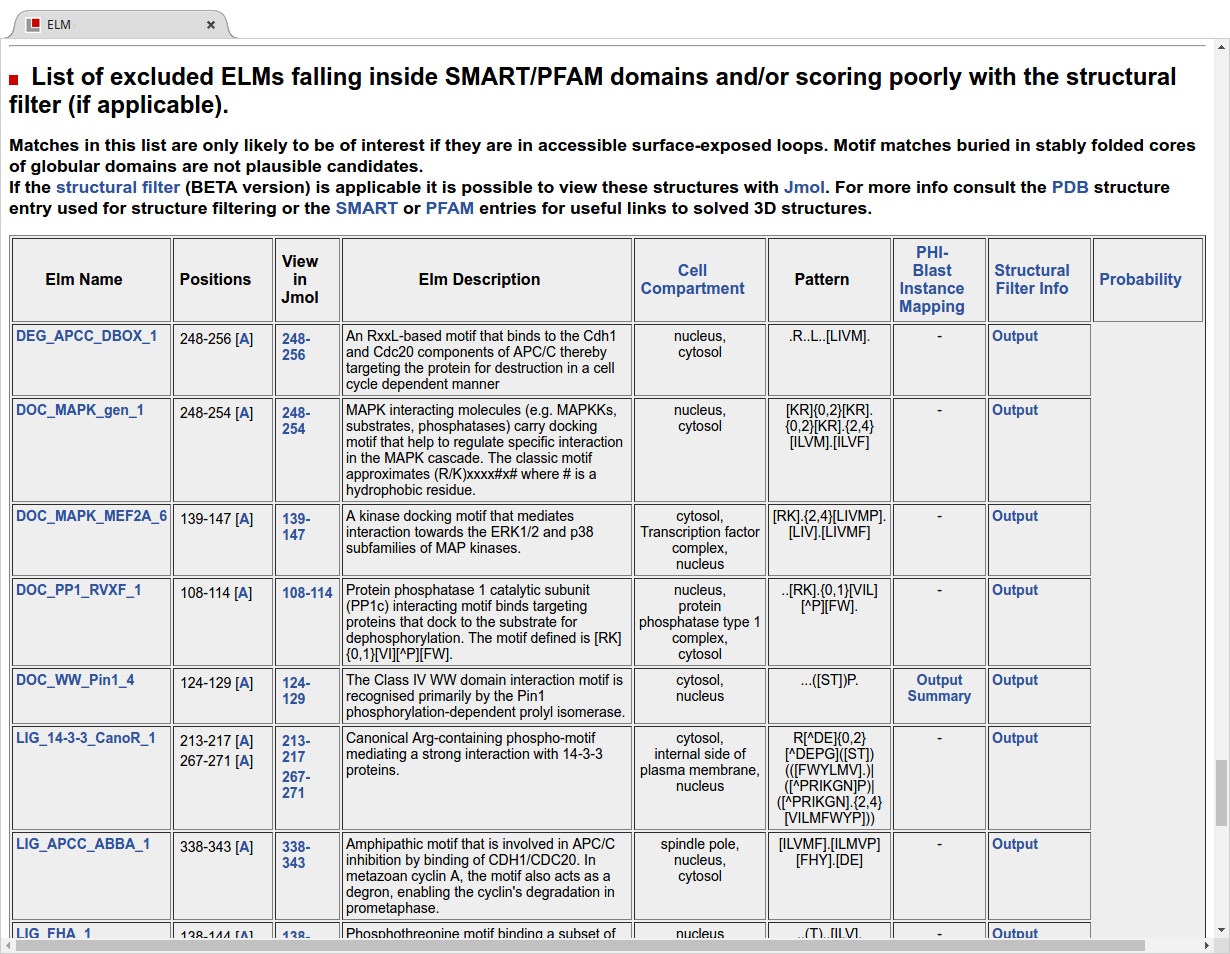
\includegraphics[width=\textwidth]{Figures/predicting_p53/elm_results_motifs_filtered.png}
	\caption{
	This table contains the list of putative motifs detected in the query sequence (only
	the top part of the table is shown) which were excluded by the
	structural or context filter.
	}
	\label{fig:predicting_p53_elm_results_motifs_filtered}
\end{figure}

\item Scroll further down to the heading ``List of excluded ELMs falling inside
	SMART/Pfam domains and/or scoring poorly with the structural filter (if
	applicable).''
	(Figure~\ref{fig:predicting_p53_elm_results_motifs_filtered})
	This table is similar to the one described above, but shows motif
	matches which were rejected by the structural filter.
\end{enumerate}

\clearpage

%%% Predicting with CV_0974
\section{Detecting Short Linear Motifs in Unknown Protein Sequences}
\label{sec:predicting_cv_0974}

% TODO: read this section to check for consistency, etc.

The ELM prediction pipeline is a very powerful way to obtain a lot of
information on which motifs are present, in which structural context they
are. However, determining which motifs are actually true positive detections
requires interpreting all of these results, as well incorporating as much
biological knowledge as possible. In this protocol we will be following a
typical example of how one might use the ELM prediction pipeline to search for
motifs in novel sequences.

Some pathogens have evolved short linear motifs in effector proteins to modify
the intracellular signalling of its host cell for its own convenience
\citep{25475989}. The Gram-negative bacteria \textit{Chromobacterium violaceum} is a
human opportunistic pathogen whose mechanism of pathogenicity remain poorly
understood. Its genome encodes a type three secretion system (T3SS) that is
used by many pathogens to translocate bacterial proteins to the infected cells.
Interestingly, the genes encoding this T3SS as well as other genes located in
the same genomic location are very similar to the ones in \textit{Salmonella spp.}
except for a couple of genes including the modular protein SptP
\citep{15100995}. SptP in \textit{Salmonella spp.} is a secreted protein tyrosine
phosphatase \citep{8866485} whose closest homolog in \textit{C. violaceum} is
the protein \uniprot{CV\_0974}. To further understand the possible biological
function of the protein \uniprot{CV\_0974} we will use it in the ELM server
detect motif.

%
% Subsection: Necessary Resources
%
\subsection*{Necessary Resources}
\subsubsection*{Software \& Hardware}
A modern browser such as Firefox, Chrome, or Safari. ELM is best viewed
on a laptop or desktop computer, although tablets and smartphones will
also work.

\subsubsection*{Files}
You need to download the following FASTA file from UniProt:
\url{http://www.uniprot.org/uniprot/Q7NZE8.fasta}

\begin{enumerate}

%
% Subsection: Submitting a query
%
\subsection*{Submitting a query to ELM}
\label{subsec:predicting_cv_0974_submitting}

\begin{figure}[h!]
	\centering
	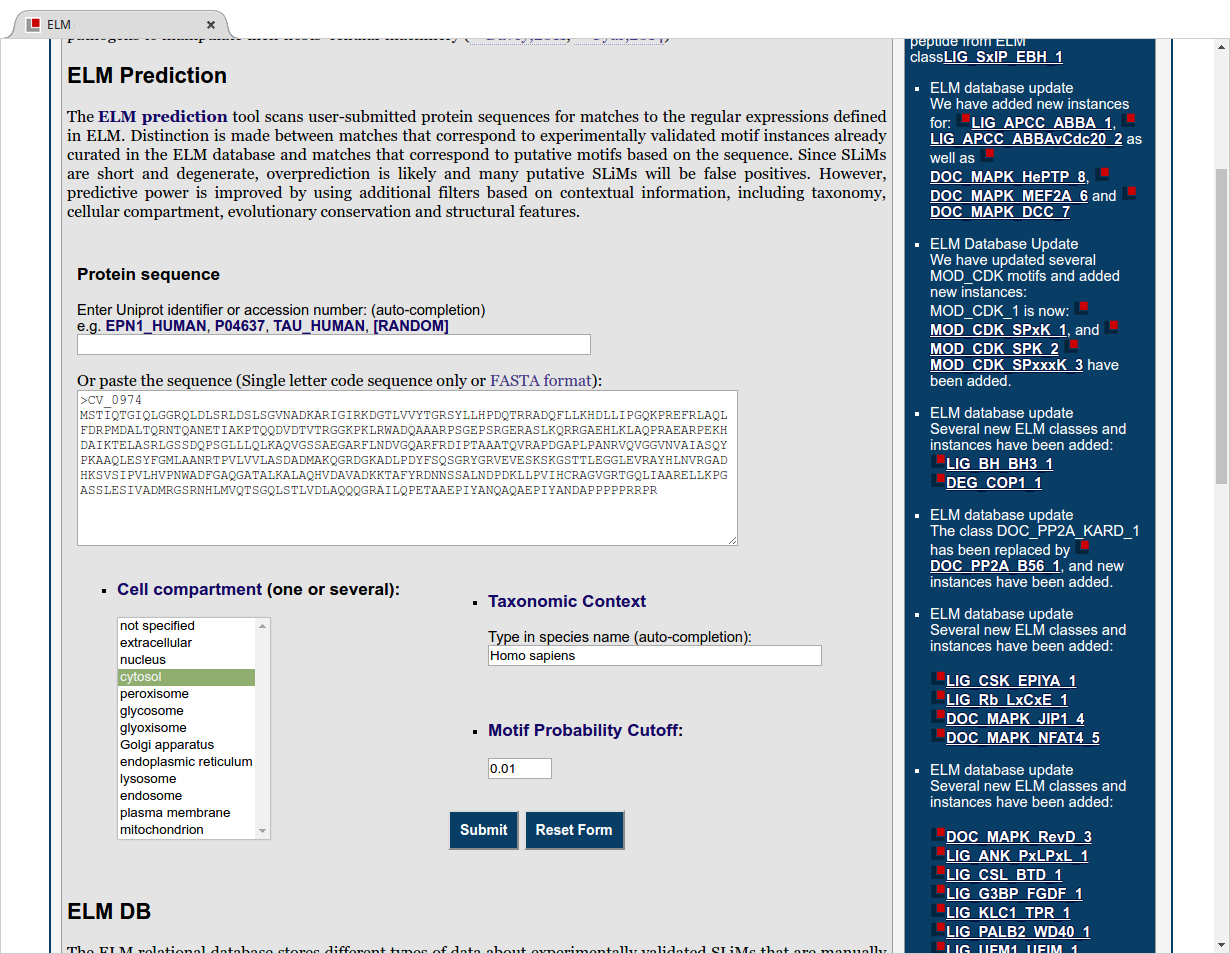
\includegraphics[width=\textwidth]{Figures/predicting_cv_0974/elm_search.png}
	\caption{
	The input query page for finding motifs in ELM. The sequence
    for \textit{C. violaceum} protein \uniprot{CV\_0974}, which is thought to be involved in its pathogenicity,
    is used as an example for this protocol.
	}
	\label{fig:predicting_cv_0974_search}
\end{figure}

\item Click on the ``ELM Predictions'' button in the menu to access the search
	query page (Fig. \ref{fig:predicting_cv_0974_search}).
	Here you can provide either a protein
	accession (from UniProt) or an amino acid sequence (simply the
	sequence, or a FASTA formatted entry) in which you want to detect
	SLiMs. Retrieve the FASTA formatted sequence from UniProt
	(\url{http://www.uniprot.org/uniprot/Q7NZE8.fasta}), and enter it into the
	``sequence input text box''.

\item In the ``Taxonomic Context'' field, start typing the text ``Homo
	sapiens''. As you type this field should auto-suggest species matching
	your text. Select ``Homo sapiens'' to limit the search to motifs
	which have been annotated in Human proteins.

	\sdesc{ Certain human diseases occur when motifs are hijacked by
		opportunistic pathogens (see Step~\ref{sec:explore_content_viruses} in
		\ref{sec:explore_content} and Figure~\ref{fig:explore_content_viruses}).
		By limiting the search to
		human motifs, we will identify motifs which are known to exist
		in humans and thus may be the target of motif hijacking.
	}

\item \uniprot{CV\_0974} is likely to be an effector protein, similarly to its
    homologue SptP. As SptP localizes to the cytosol, we can assume the same
    for \uniprot{CV\_0974}. Select ``cytosol'' in the ``Cell compartment''
    field.

\item Lastly we will change the ``Motif probability cutoff value'' to a more
	stringent threshold. Enter ``0.01'' for this value. This will exclude
	all motif with a probability score higher than ``0.01'', limiting the
	results to motifs which are more likely not to represent random
	sequences of amino acids.

\subsection*{Interpreting the results}
\label{subsec:predicting_cv_0974_submitting}

\begin{figure}[h!]
	\centering
	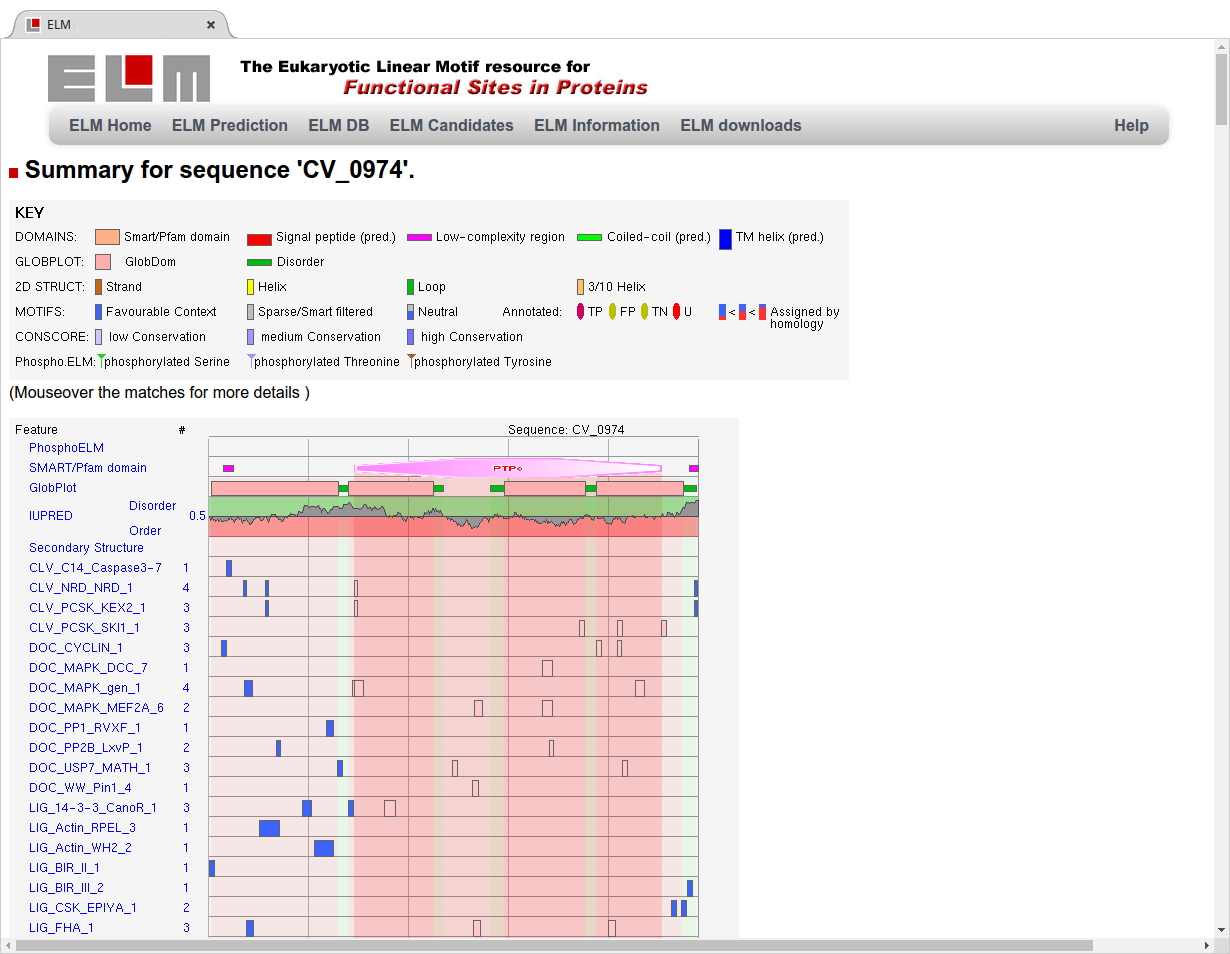
\includegraphics[width=\textwidth]{Figures/predicting_cv_0974/elm_results_summary.png}
	\caption{
	The graphical results summary of the ELM Prediction pipeline for
	Probable Tyrosine phosphate (\uniprot{CV\_0974}). Note that not all motif
	detections are shown (the image is truncated at the bottom). The top
	five rows show a handful of structural features. The motif occurrence
	are shown as blue boxes, the intensity of which indicates the
	conservation score. See steps
	\ref{sec:predicting_p53_results_phosphorylation} to
	\ref{sec:predicting_p53_results_structure_filter} of
	\ref{sec:predicting_p53}
	for more information.
	}
	\label{fig:predicting_cv_0974_results_summary}
\end{figure}

%
% Subsection: Understanding results: graphical summary
%

\subsection*{Interpreting the prediction results}
\label{sec:predicting_cv_0974_graphical_summary}

\item Hit \button{Submit} to send the query to the ELM prediction pipeline.
    The Results are summarized in the first figure on the results page
	(see Fig. \ref{fig:predicting_cv_0974_results_summary})
    See steps \ref{sec:predicting_p53_submit} -- \ref{sec:predicting_p53_results_structure_filter} 
    of \ref{sec:predicting_p53} for a description of the
    graphical summary output.

\item Find the entry for \motif{LIG\_CSK\_EPIYA\_1} in the graphical summary.
    When this motif is tyrosine-phosphorylated it is recognized by C-terminal
    kinase. Different effector proteins from human pathogens like
    \textit{Bartonella henselae}, \textit{Helicobacter pylori} and
    \textit{Haemophilus ducreyi} have been reported to use this motif to
    interfere with the host signalling network to induce proliferation or to
    avoid phagocytosis \citep{19380118, 12446738, 24902122}.

\item Check the structural context for both \motif{LIG\_CSK\_EPIYA\_1} motifs
    predicted in \uniprot{CV\_0974}. Both of them fall outside of the SMART
    domain PTPC, and reside in a region with a protein disorder (IUPred) score
    above 0.5. Both of these conditions are indicative that these motifs might
    be True Positive predictions.

    \sdesc{You may notice that there are no conservation scores for either of
        these motifs. A closer examination of the alignments of homologous
        proteins shows that none of the other proteins have this part of the
        sequence, and are gapped, thus it is not possible to calculate a
        conservation score.}

\item Click on the motif identifier \button{LIG\_CSK\_EPIYA\_1} in the
        graphical summary to be brought to the motif details page for this
        motif. In the ``Functional site description'' it is stated that 'The
        bacterial proteins usually have repeats of EPIYA motifs.' The ELM
        prediction results did indeed also detect two EPIYA motifs in a 20
        amino acid range, lending further support to the likelihood that there
        are indeed two functional EPIYA motifs in \uniprot{CV\_0974}, which in
        turn suggests that these motifs may be involved in \textit{C.
        violaceum's} pathogenicity.

\end{enumerate}

\clearpage

%%% Searching via REST API
\section{(Alternative Protocol) Searching the ELM database using the REST API}
\label{sec:search_REST}

Many researchers are interested in large-scale analyses rather than
information about individual protein sequences. To this end, individual
queries to the ELM webserver with a single protein id at a time, are not
practical.

For this reason, as much information as possible is made available via a
REST interface \citep{Fielding2002}. This allows the user to interact
with the ELM database and ELM webserver via scriptable URL requests.
Each request can easily be tested in the browser before it is being
automated in a script.

In this section we will explore the various ways in which data can
downloaded both in using the browser as well as via the commandline.

%
% Subsection: Necessary Resources
%
\subsection*{Necessary Resources}
\subsubsection*{Software}
A modern browser such as Firefox, Chrome, or Safari. ELM is best viewed
on a laptop or desktop computer, although tablets and smartphones will
also work.
%
There exist several REST client plugins for different browsers, however these
are not needed for this protocol. Ideally use a commandline tool such as
\cl{curl} (\url{http://curl.haxx.se/}) in a terminal window. This program is
available in any of the major operating systems: OSX, Windows and Linux. Of
course, \cl{curl} is only one of many different ways to access web content
programatically, and we suggest to use whichever program you feel is
better suited for your tasks.



\begin{enumerate}

%
% Subsection: Necessary Resources
%
\subsection*{Downloading all ELM
classes}\label{downloading-all-elm-classes}

\begin{figure}[h!]
	\centering
	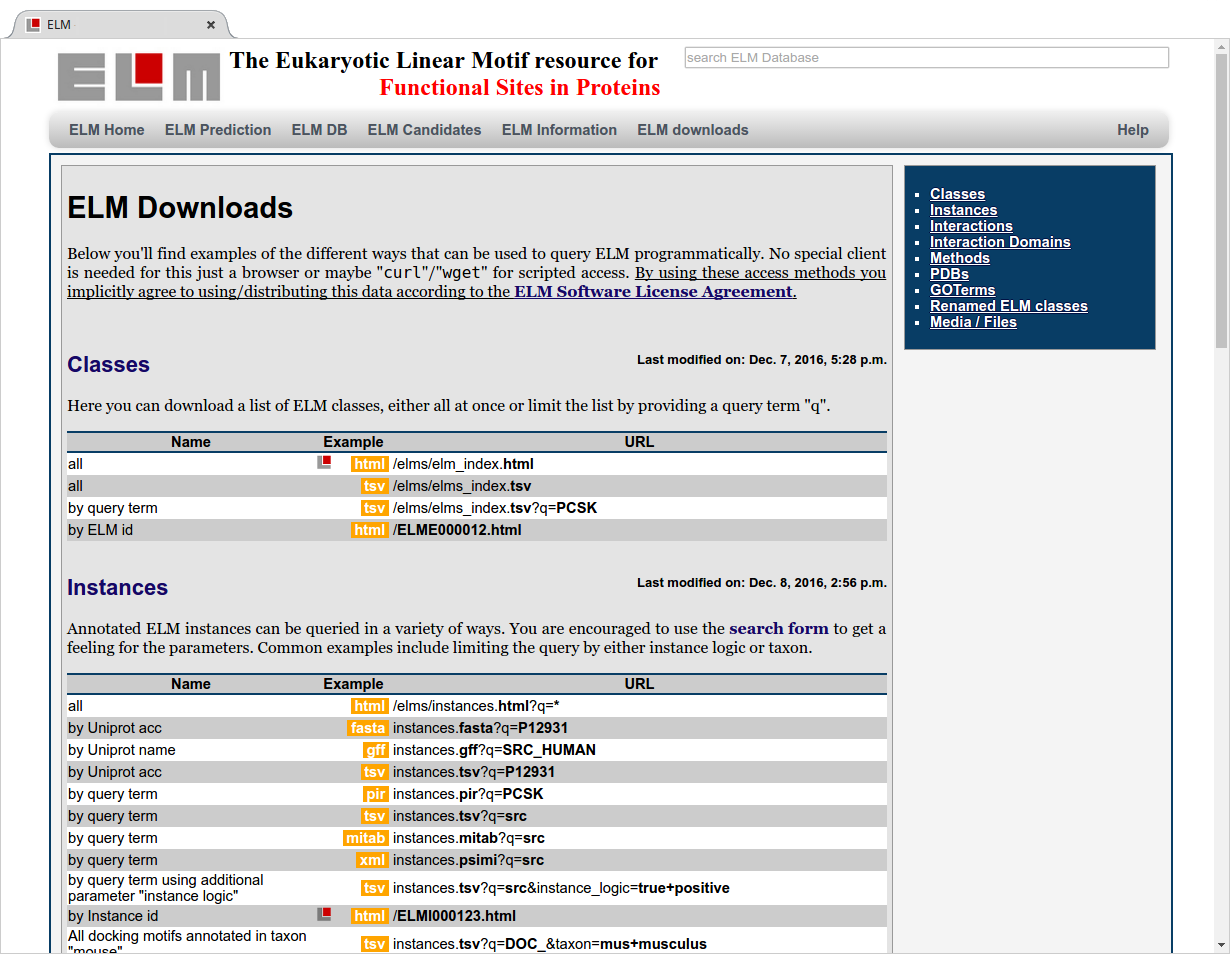
\includegraphics[width=\textwidth]{Figures/search_REST/elm_downloads_html.png}
	\caption{
	The ELM downloads page, which holds
	information about the different types of data (such as ``Classes'',
	``Instances'', etc; see menu to the right) that can be obtained from the
	server. The orange boxes are clickable links, the URL following them are
	used to highlight the URL scheme used by the server (bold font denotes
	specifics used in the examples such as query terms, or formats).
	}
	\label{fig:search_REST_downloads}
\end{figure}

\item Direct your browser to the URL '\rurl{elm.eu.org/downloads}' or select
    \button{ELM Downloads} from the main menu
	(Figure~\ref{fig:search_REST_downloads}).
	This page contains links and descriptions on how to download ELM data
	in text format. The datasets are split into several smaller collections
	(for example ``Classes'', ``Instances'', etc). Each table contains
	links (in orange) to download the data in appropriate formats.

	\sdesc{Each table also shows the `last modified date' indicating when
		the data was last updated. This information is useful if you want to know
		when to update your local data with the most up to date ELM
		data as it allows you to determine whether you need to update or not. }

\item Click on the first orange \button{html} link in the table ``Classes'' to
	navigate to the following URL:
	'\rurl{elm.eu.org/elms/elm\_index.html}'. This page shows all of the
	annotated ELM classes in the database. This page is the same one as
	shown in Figure~\ref{fig:explore_content_elms}. 

\item Navigate to the following URL: '\rurl{elm.eu.org/elms.html?q=CSK}'
	specifying \cl{q=CSK} to limit the list of ELMs to those matching the
	search query ``CSK''. This page is again similar to the one shown in
	Figure~\ref{fig:explore_content_elms}, but with less classes.

	\sdesc{ This search result is identical to the result you would obtain
		by doing a ``manual'' search on the ELM Classes page
		(eg. typing 'CSK' in the search box and clicking \button{submit}) as
		described in step \ref{sec:predicting_p53_submit} of \ref{sec:explore_content}
		(see Figure~\ref{fig:explore_content_elms}).}


\item Open the following URL: '\rurl{elm.eu.org/elms.tsv?q=CSK}' to download a
	list of classes that match the search query ``CSK'' (as in the previous
	step) in the ``tab separated values'' format. Note that this time we
	used the file extension '.tsv' instead of '.html' as before. By
	exchanging the '\fileformat{.html}' part of the URL with
	'\fileformat{.tsv}', we ask the webserver to give us the data in
	``tab-separated values'' format.

	\sdesc{ Depending on which browser you are using, the file may open
		directly in your browser, or you may be prompted to download
		the file or save it to a separate location. In the latter two
		cases you can open the downloaded file using a (plain) text
		file viewer, or possible a spreadsheet viewer (such as
		Microsoft Excel or LibreOffice Calc).}

\begin{figure}[h!]
	\centering
	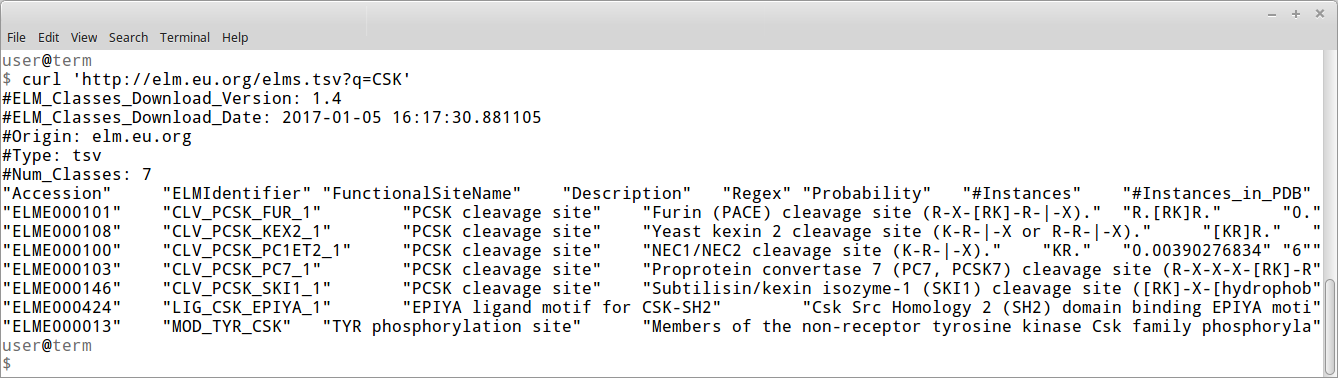
\includegraphics[width=\textwidth]{Figures/search_REST/elm_curl_classes_CSK.png}
	\caption{
	A screenshot of a terminal window using
	\cl{curl} to download all ELM classes matching the term `CSK'.
	}
	\label{fig:search_REST_curl_csk}
\end{figure}

\item Type the following command into a command line terminal to
	download the same data from the previous step directly into the
	terminal:
	\cl{curl 'http://elm.eu.org/elms/elms\_index.tsv?q=CSK'}. The output
	should look similar to Figure~\ref{fig:search_REST_curl_csk}.
	The column names are the same as shown in Figure~\ref{fig:explore_content_elms}.

	\sdesc{ Use the curl option ``\cl{-o}'' to save the results directly to
		a file. For example: \cl{curl -o classes.tsv
		'http://elm.eu.org/elms/elms\_index.tsv?q=CSK'} will save the
		data to a file called \emph{classes.tsv}.}

\begin{figure}[h!]
	\centering
	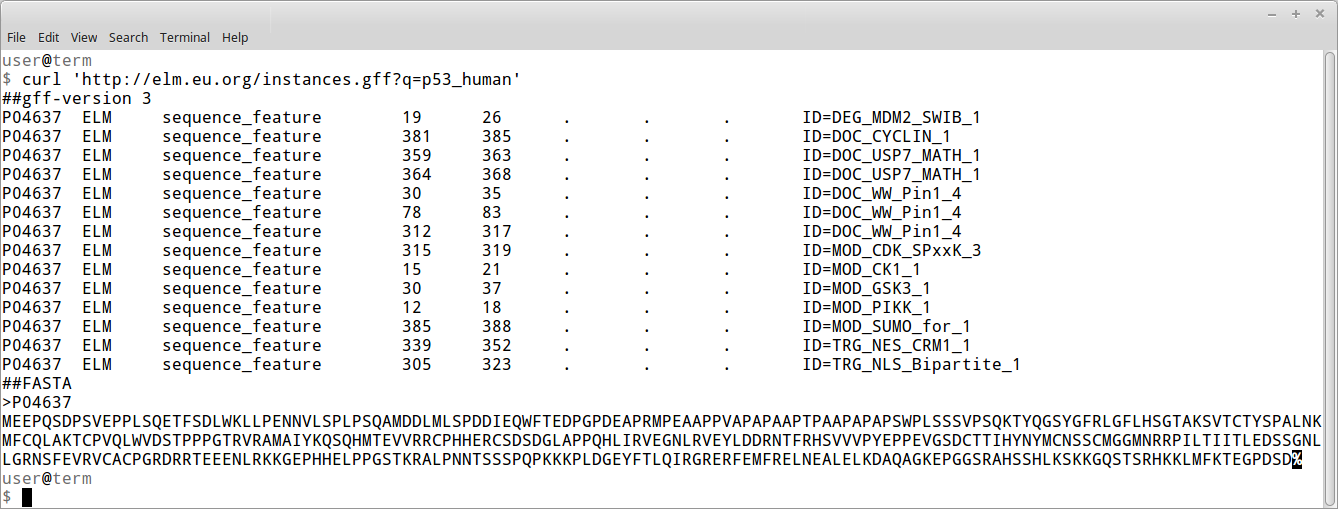
\includegraphics[width=\textwidth]{Figures/search_REST/elm_curl_instances_p53_human.png}
	\caption{
	Screenshot of a terminal window using \cl{curl} to download all ELM
	instances annotated for sequence P53\_HUMAN.
	}
	\label{fig:search_REST_curl_p53}
\end{figure}

\item To download a list of all motif instances detected in the protein sequence of human p53, type the
	following command into a terminal: \cl{curl
	'http://elm.eu.org/instances.gff?q=p53\_human'}. The output should look
	similar to that shown in Figure~\ref{fig:predicting_REST_curl_p53}. The
	output is in the ``General Feature Format''
	(see \rurl{www.ensembl.org/info/website/upload/gff.html\#moreinfo}),
	with the FASTA formatted sequence appended to the end of the output.

	\sdesc{Many other file formats are available for downloading instances
	annotations; see the downloads page for available options including the 
	\fileformat{FASTA}, \fileformat{GFF},
	\fileformat{PIR}, or \fileformat{PSI-MI} format (either
	\fileformat{XML} or \fileformat{MiTab}). 
	}


\item To download a list of all instances matching the search query ``CLV'' annotated for the taxon
	``yellow fever mosquito (\textit{Aedes aegypti})'', enter the following
	command into a terminal:
	\cl{curl `http://elm.eu.org/instances.tsv?q=CLV\&taxon=aedes+aegypti'}
	(In general, any species name can be used, however remember to replace all ``spaces''
	with ``+''). This should return a single instance, the only one
	matching \motif{CLV} in \textit{A. aegypti}.

\item More data (interactions, domains, methods, etc.) can be downloaded from
	ELM in analogous fashion as shown in the preceding steps. Take a look
	at the ELM Downloads page (\rurl{elm.eu.org/downloads}, figure
	\ref{fig:search_REST_downloads}) for an overview of which datasets can
	be downloaded, and what different filters and formats are available
	for each dataset.

\end{enumerate}

\clearpage

%%% Predicting via REST API
\section{(Alternate Protocol) Detecting Short Linear Motifs in Sequences using the REST API}
\label{sec:predicting_REST}

Querying ELM for motifs in a given sequence (as described in
\ref{sec:predicting_p53} and \ref{sec:predicting_cv_0974}), gives you a nice
overview of putative and possibly
annotated motifs in your query protein with a graphical representation
using colors to highlight different regions of the protein sequence (eg.
disordered vs. globular). It is however difficult to analyse a large set
of protein sequences in this manner. Therefore, the ELM server
provides an interface which you can use to submit your sequence in a
programmatic way. Of course, this way, you won't receive the graphical
output representation, but are limited to textual data representation.

Currently, there exists a single URL (\rurl{elm.eu.org/start\_search/})
to accept such queries. You can choose to either submit a UniProt name
or accession (eg. '\url{elm.eu.org/start\_search/P53\_HUMAN.tsv}') or
submit your raw sequence (e.g. '\rurl{elm.eu.org/start\_search/MAPRGFSCLLLLTSEIDLPVKRRA}'.)
If the URL ends in `.tsv' then the server assumes you
are using a UniProt id or accession; if it doesn't, then it assumes you
are using raw sequence. See below for details.

%
% Subsection: Necessary Resources
%
\subsection*{Necessary Resources}
\subsubsection*{Software}
A modern browser such as Firefox, Chrome, or Safari. ELM is best viewed
on a laptop or desktop computer, although tablets and smartphones will
also work.
%
There exist several REST client plugins for different browsers, however these
are not needed for this protocol. Ideally use a commandline tool such as
\cl{curl} (\url{http://curl.haxx.se/}) in a terminal window. This program is
available in any of the major operating systems: OSX, Windows and Linux. Of
course, \cl{curl} is only one of many different ways to access web content
programatically, and we suggest to use whichever program you feel is
better suited for your tasks.

%
(Note that in some of the following screenshots, we append the following
command to the commandline ``\cl{| column -t}'' to make the output more
readable. All this does is to properly align all columns at tabstops.)

\begin{enumerate}

%
% Subsection: Submitting a query via the REST API
%
\subsection*{Submitting a query to ELM via the REST API}
\label{subsec:predicting_REST_submitting}

\begin{figure}[h!]
	\centering
	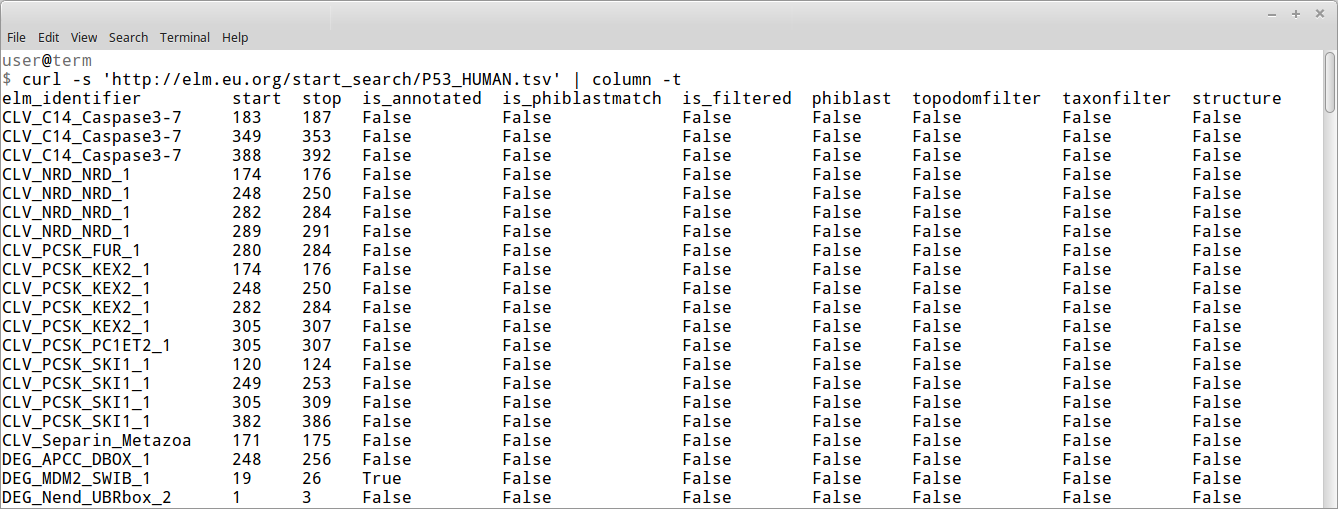
\includegraphics[width=\textwidth]{Figures/predicting_REST/curl_P53.png}
	\caption{
	The commandline output when \cl{curl} is used to
	download all motifs predicted in human p53.}
	\label{fig:predicting_REST_curl_p53}
\end{figure}


\item Use \cl{curl} to query ELM for all motifs predicted to occur in human
    p53 by typing the following into a terminal: `\cl{curl
	`http://elm.eu.org/start\_search/P53\_HUMAN.tsv}'.
	See Figure~\ref{fig:predicting_REST_curl_p53} for example output.
	Each resulting row represents a
	motif detection, and the first column ``elm\_identifier'' indicates
	which ELM class was identified, multiple matches to the same class are represented in multiple lines.
	The columns ``start'' and ``stop'' show
	that first and last amino acid positions that matched the motif.
	The column ``is\_annotated'' is True if this motif has been
	annotated in the ELM database as an (experimentally validated) motif
	instance. The column ``is\_phiblastmatch'' is True if a match was found
	by the ELM Instance mapper indicating that an experimentally validated
	instance in a homologous sequence was found
	(see commentary section "Instance Mapper" at page \pageref{InstanceMapper}).
	The column ``is\_filtered'' shows whether or not this motif was rejected by any
	of the ELM prediction filters (structure, topodom, taxon), whereby
	``topodomfilter'' uses information from UniProt to determine the protein's ``topology''
	with respect to trans-membrane domains or extracellular regions.
	The columns ``taxonfilter'' and ``structure'' indicate that an instance
	has been filtered by the taxonomy or secondary structure filter, respectively
	(see commentary sections "Taxon Filter" and "Structure Filter" 
	%at page \pageref{TaxonFilter}
	).

	\sdesc{In FigureF\ref{fig:predicting_REST_curl_p53}
		we use a slightly more
		advanced command to get the output to look nice in the
		terminal. We specified the \cl{-s} option to silence all
		\cl{curl} output other than the downloaded file, and piped
		the output directly to the
		\cl{column} command (this command exists on most Liux and
		OSX machines).}



\begin{figure}[h!]
	\centering
	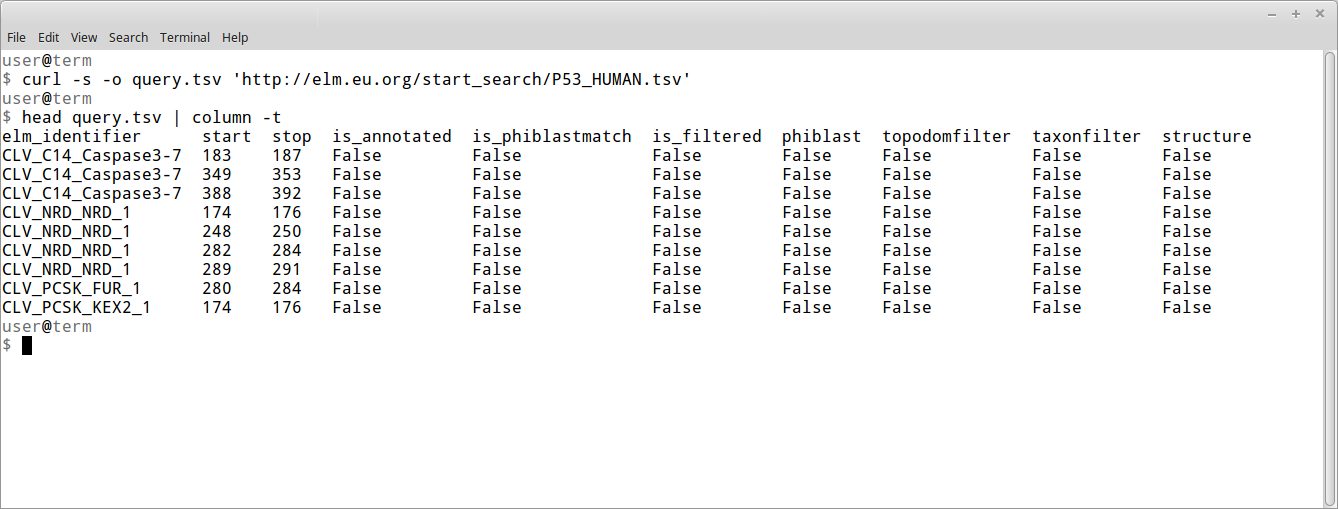
\includegraphics[width=\textwidth]{Figures/predicting_REST/predictions_query.png}
	\caption{
	It is possible to send amino acid sequences to the ELM Prediction
	pipeline. In this case we have used
	the curl option ``\cl{-o}'' to download directly to the file
	\cl{query.tsv}, and use a combination of the \cl{head} and
	\cl{column} commands to display the first 10 rows to the terminal.
	}
	\label{fig:predicting_REST_query}
\end{figure}

\item Use \cl{curl} to query ELM via protein sequence by using the URL
	'\rurl{elm.eu.org/start\_search/MAPRGFSCLLLLTSEIDLPVKRRA}'
	(Figure~\ref{fig:predicting_REST_query}).
	In this case the query is an arbitrary short
	peptide sequence, but this can (of course) contain any sequence you are
	interested in analysing. The output format is exactly the same as in the
	previous step.

	\sdesc{ This way of querying ELM is unfortunately not stable for long
		protein sequences. Different browsers and computers have
		different maximum lengths for URLs, and the excess text is
		often simply ignored. We recommend not using this method for
		sequences longer than 2000 amino acids.}

\end{enumerate}

\clearpage

%%% Commentary
\section*{Guidelines for Understanding Results}
\label{sec:guidelines-for-understanding-results}

Marc: TODO: Still working on this bit.

The annotations in the ELM database have all been selected and In most cases
you can safely assume that the annotations present in the database are all of
high confidence.
These annotators have a lot of exprience in reading the scientific literature,
and know how to distinguish high confidence from suggestive expriments
\cite{26581338}.
You are also encouraged to dig deeper into each annotation.
In all cases each entry contains descriptions of the expriments performed and
links to the original reasearch.

Understanding the results generated by the ELM prediction pipeline 
can sometimes require some extra work.
In \ref{sec:predicting_p53} and \ref{sec:predicting_cv_0974} we gave a few
examples of how to read and interpret the results from the ELM prediction
pipleline.
These are bioinformatics predictions, and therefore will rely
on a heuristic which will make mistakes.
In general the  prediction pipeline attempts to make as many predictions as
possible, at the risk of making some False Positive predictions as well.

In cases all of the intermediarte results generated by the ELM prediction
pipeline are made available to aid you in deciding which preditions are worth
further investigation.
Looking at the multiple sequence alignments used to generate the conservation
score can (for example) help determine why a seemingly likely motif may have a
(falsely) low confidence score.
On the contrary you may have reason to belive that a predicted motif that was
rejected by ELM's structure filter may actually exposed in a different
structural conformation. 


\emph{instructions: A brief discussion of the theory and applications of
your}

\emph{notes: Maybe mention how findings are relevant to the lab? For
example: Manually annotated content should be reliable, although one
should look at the `confidence' in the instance annotation. Predictions
are probably trustworthy, but you need to take into account the
`confidence score', and other features like whether its in a domain,
etc\ldots{}}

\section*{Commentary:}\label{commentary}

\emph{instructions: A brief discussion of the theory and applications of
your}

\subsection*{Background Information}\label{background-information}

In order to interpret the data contained in ELM and the results produced by the
ELM prediction tool, it is important to have a basic understanding of SLiM's
and how they are affected by their structural and biological context. This
background information summarises the different functionalities of SLiMs,
describes the degenerate nature of motif sequences, and emphasises the need for
contextual data for confident SLiM prediction.

\subsubsection*{ELM categorises SLiMs depending on their functionality}

SLiMs mediate different types of interactions, and based on this functionality,
the ELM classes annotated in the ELM database are grouped into six main ELM
types (Figure~\ref{fig:SLiMclasses}, \cite{24214962}). They can function as ligand binding sites or
as sites for post-translational modification (PTM). Some ligand SLiMs are
recognised by components of the cellular transport machinery and function as
localisation signals that target proteins to specific sub-cellular compartments
(\motif{TRG} type). Other ligand SLiMs are abundantly present in interfaces that mediate
the assembly of large macromolecular complexes and in highly modular scaffold
proteins that act as multivalent platforms for protein complex assembly
(\motif{LIG} type). Docking motifs are ligand SLiMs that recruit modification enzymes to
their substrates by binding to a site on the enzyme that is distinct from the
active site (\motif{DOC} type). A subset of these, known as degrons, recruit ubiquitin
ligases, which subsequently polyubiquitylate their substrates and hence target
them for proteasomal degradation (\motif{DEG} type). SLiMs that act as sites for PTM can
be targeted by specific enzymes for the addition or removal of a small chemical
group (e.g. phosphorylation), a sugar molecule (e.g. glycosylation), a protein
(e.g. ubiquitylation), or another moiety (e.g. lipidation) (\motif{MOD} type). Other PTM
SLiMs mediate proteolytic cleavage by acting as target site for proteolytic
enzymes (\motif{CLV} type), or are recognised for structural modification by isomerases
that catalyse cis-trans isomerisation of the peptide backbone (\motif{DOC} type), see
\cite{24926813} and \cite{24773235}.

\subsubsection*{ELM regular expressions reflect the degenerate nature of SLiMs}

As their name suggests, SLiMs are compact, being composed of a limited number of
adjacent amino acids. Most of a motif's binding specificity however is conferred
by only a subset of these amino acids. Those few residues that directly interact
with the binding partner are evolutionary conserved, although in many cases a
subset of amino acids that share certain properties (such as similar charge,
size or hydrophobicity) are allowed in these hotspot positions. In the motif
positions that contribute little to the interaction, there are even less
constraints, i.e. a broader range of amino acids is allowed in these positions
\citep{21909575}. This sequence flexibility is captured in the regular
expressions that are defined for each motif class. A first consequence of this
degeneracy is that SLiMs co-operatively engage in interactions of relatively low
affinity. Hence these binding events are transient and reversible, and can be
readily modulated, for instance by PTM. These characteristics make SLiM-based
interactions ideal mediators of the dynamic processes involved in cell
signalling \citep{22480932}. Another consequence is that it might take only a few
or even a single point mutation to generate or disrupt a functional motif in a
protein. The associated ability to evolve convergently might underlie the
proliferation of SLiMs and the rewiring of interactomes \citep{26589632,
22346764}. Conversely, several SLiM-associated diseases have been
characterised to date, for instance Liddle syndrome \citep{15483078}.

\subsubsection*{ELM integrates data to increase the confidence of SLiM prediction}

Due to their degenerate nature, motif sequences contain only very little
information, and many short sequences in a proteome will match motif patterns.
However, most of these matches will not represent functional motifs, and hence,
when scanning a proteome for putative motifs using only the motif sequence
patterns will yield a large number of false positive instances, far exceeding
the number of true motifs. Therefore, reliable motif detection cannot go without
experimental validation of candidate motifs, using different types of
experiments and techniques \citep{26581338}. This however does not mean that
bioinformatics analysis cannot guide researchers towards a subset of candidate
motifs that have a higher probability to be functional and help rule out those
candidate motifs that are likely to be false positives. Taking into account
additional information, besides a match to a sequence pattern defining a SLiM,
can greatly narrow the selection of putative motifs for experimental validation.
Additional data for in silico analysis include conservation of the motif
sequence, the location of the motif within the protein's structure and its
accessibility for its binding partner, validated interaction with the binding
partner, and in-cell co-localisation with the binding partner. The availability
and usefulness of these additional data for SLiM discovery depends on their
extensive and correct biocuration. A vast and increasing amount of biological
data is available in a wide variety of sources, including the literature and
large-scale datasets. In order to facilitate integration of data, they need to
be collected, annotated and formatted in central data and knowledge
repositories. The ELM database provides such a repository for experimentally
validated linear motif classes and instances. The ELM prediction tool in turn
relies on annotated data, both from the ELM database and other resources, to
accurately analyse unknown sequences for candidate motifs and assist researchers
in selecting the most plausible ones for experimental validation and discard
likely false positive hits, saving them valuable time and assets
\citep{22110040}.

\subsubsection*{ELM Filters}

\paragraph*{Disorder Filter}\label{DisorderFilter}

ELM uses two different predictors of globularity/disorder: Firstly, GlobPlot
developed by \cite{12824398}, uses amino acid propensities derived from a set of
proteins to detect regions of globularity/disorder in any given protein
sequence. Secondly, IUPred by \cite{15955779}, which, unlike GlobPlot, has not
been trained on any dataset, but rather uses a position-specific scoring scheme
assessing the tendency of any given amino acid to reside in either an ordered
or disordered region. IUPred assigns a score between 0.0 to 1.0 to each amino
acid of a protein sequence, whereby protein segments with an IUPred score above
0.5 are considered to be disordered. ELM displays IUPred scores as a colored
line on either green (disordered) or red (globular) background, see rows four
and five of Figure~\ref{fig:predicting_p53_results_summary}.

\paragraph*{Structure Filter}\label{StructureFilter}

The structural filter, especially developed for ELM by \cite{19852836},
assesses accessibility and secondary structural context derived from
experimentally solved protein structures. It maps putatively functional motif
occurrences onto a representative domain structure and scores these motifs for
solvent-accessibility and secondary structure context. ELM displays this
information as overlay boxes in the graphical output, whereby the user needs to
hover over individual instance entries within structural context (see the
\motif{CLV\_PCSK\_SKI1\_1} example in fig.
\ref{fig:predicting_p53_results_summary}).

\paragraph*{Conservation Filter}\label{ConservationFilter}

This filter method for scoring the conservation of linear motif instances was
developed by \cite{18460207} and subsequently implemented into the ELM
pipeline. It requires only primary sequence-derived information (e.g. a
multiple alignment and the sequence tree) and implicitly takes into account the
degenerate nature of short linear motif patterns. By auto-generating multiple
sequence alignments from a non-redundant database, generating distance-trees
and taking into account motif degeneracy, it assesses for each ELM motif class
found in any given sequence its conservation. The conservation score ranges
from 0.0 (the predicted instance is present only in the query sequence) to 1.0
(full conservation of the motif regular expression in all the informative
sequences).

Since conserved motifs in structural regions are most likely conserved for
structural integrity rather than motif function, one always has to assess the
context when inspecting conservation score. Generally, best motif candidates
are those with high conservation scores in regions of unstructured, unconserved
regions.

% When investigating conservation of short linear motifs, one has to bear in mind
% Further generalizing, taking into
% account that the more likely it is a functional motif for this prediction.
%
% islands of conservation amidst a sea of unconserved disordered amino acid residues.

\paragraph*{Taxon Filter}\label{TaxonFilter}

Each ELM class is annotated with one or more taxonomic ranges, for which
experimental evidence has been found for the particular class
(see "Present in Taxon: Eukaryota" in figure
\ref{fig:explore_content_doc_cyclin}). This information is then used to filter taxons
outside the annotated range whenever a user submits a query sequence to the ELM
database (see the \button{taxonomic context} field in the ELM search input form in fig.
\ref{fig:predicting_p53_elm_search}).

\paragraph*{Instance Mapper}\label{InstanceMapper}

The ELM instance mapper takes all annotated instances from the ELM database,
generates a BLAST database from it and uses \cl{phiblast} to detect sequence stretches in
the query sequence which are similar to sequences in this database. This allows
the instance mapper to effectively map known instances (for which experimental
evidence exists) onto homologous sequences of unknown function.

%TODO: cite PHiblast?     PMID:2231712

\begin{figure}[h!]
\centering
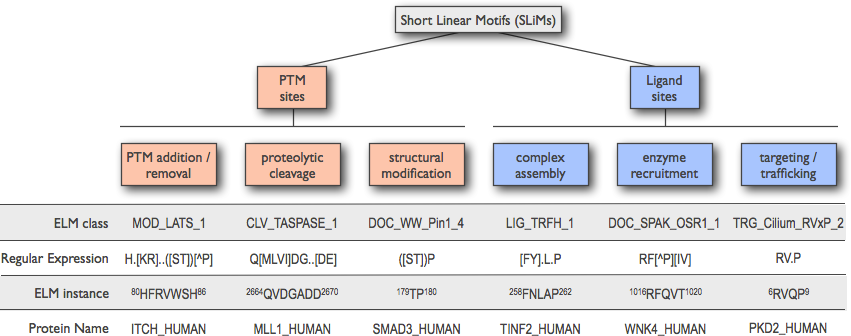
\includegraphics[width=\textwidth]{Figures/Introduction/functional_classification_of_SLiMs.png}
\caption{
For each ELM class, the
functional category to which it belongs is indicated by a three-letter prefix.
Each ELM class is defined by a regular expression. Peptide sequences in
proteins that match the regular expression of a specific ELM class and that
were experimentally validated to be functional motifs are captured as ELM
instances of that class. Degrons are a specific subtype of enzyme-recruiting
docking motifs (see text for a detailed description).
}
\label{fig:SLiMclasses}
\end{figure}

\subsection*{Critical Parameters and Troubleshooting}\label{critical-parameters-and-troubleshooting}

\emph{Factors that influence the protocol and to which special attention should be paid.
Common problems with the protocols, their causes, and potential solutions. The information may be presented in tabular form or it may be combined with Critical Parameters.
}

\section*{Internet Resources with Annotations}%
\label{internet-resources-with-annotations}

http://www.clustal.org/omega Clustal Omega \citep{21988835} is a tool
for the alignment of multiple nucleic acid and protein sequences.

http://www.jalview.org Jalview \citep{19151095} is a Java desktop
application (and browser applet) that employs web services for sequence
alignment and visualization.

http://proviz.ucd.ie ProViz \citep{27085803} is an interactive protein
exploration tool, which searches several databases for information about
a given query protein. Data relevant to the protein like an alignment of
homologues, linear motifs, post translational modifications, domains,
secondary structure, sequence variations and others are graphically
represented relative to their position in the protein.


\bibliography{references}

\end{document}
